\chapter{Overview of the oscillators/energy levels framework}
The o/el framework and conventional frameworks offer very different conceptualizations of “syntax”. In conventional approaches, a syntax “module” builds “structures” of “objects” which map both to speech motor output and to a meaning representation. This modular approach separates syntax from the phenomena that are most directly important for communication: movements/sensory experiences (a.k.a. the sensorimotor interface, phonological form), and meaning experiences (a.k.a. the conceptual-intentional interface, logical form). The modular interface view encourages us to see syntax as independent from meaning and independent from movement/sensation. We should reject this way of thinking. Syntax should not be understood as a module, but as a generic term for mechanisms which organize meaning and sensorimotor experience. Experiences are highly ordered states, and syntax is a mechanism for creating order. 

  The o/el framework rejects modules and instead embraces the notion of a \textit{system}. A system is a portion of the universe associated with some partially predictable mapping from input information to output information. In the o/el conception there are many systems, of two fundamental types: concept systems and syntactic systems. Unlike the weak, unidirectional interfaces of modules, o/el systems may have strong, bidirectional interactions. Even more importantly, o/el systems do not operate on structures of “objects”. Instead, concept systems and syntactic systems have states and exert forces on one another. Below we develop a detailed picture of these systems and their interactions. 

  An important way in which the current approach differs from conventional ones is that we attempt to motivate the framework with inferences based on knowledge of neural population dynamics. The o/el framework is derived from a microscopic conceptualization in which population coding and interpopulation connectivity play major roles in determining behavioral patterns. There are many ways in which our derivation of a macroscopic analysis relies on incomplete information and unsubstantiated assumptions regarding the microscale; I accept the possibility that invalidation of the microscale assumptions may compromise the framework.

\section{Concept systems}

How do complex patterns of thought arise in the brain? For example, consider the sentence \textit{Al drinks coffee}. In the conventional metaphor, a phrase is a “structure of objects” that arises from the merger of smaller objects. These objects—words and phrases, i.e. “linguistic units”—are also the sort of objects that can be “containers”. Thus words contain meaning and phrases contain words. Connected object representations as below use vertical orientation and connection schemas to encode these containment relations:

  
\begin{figure}
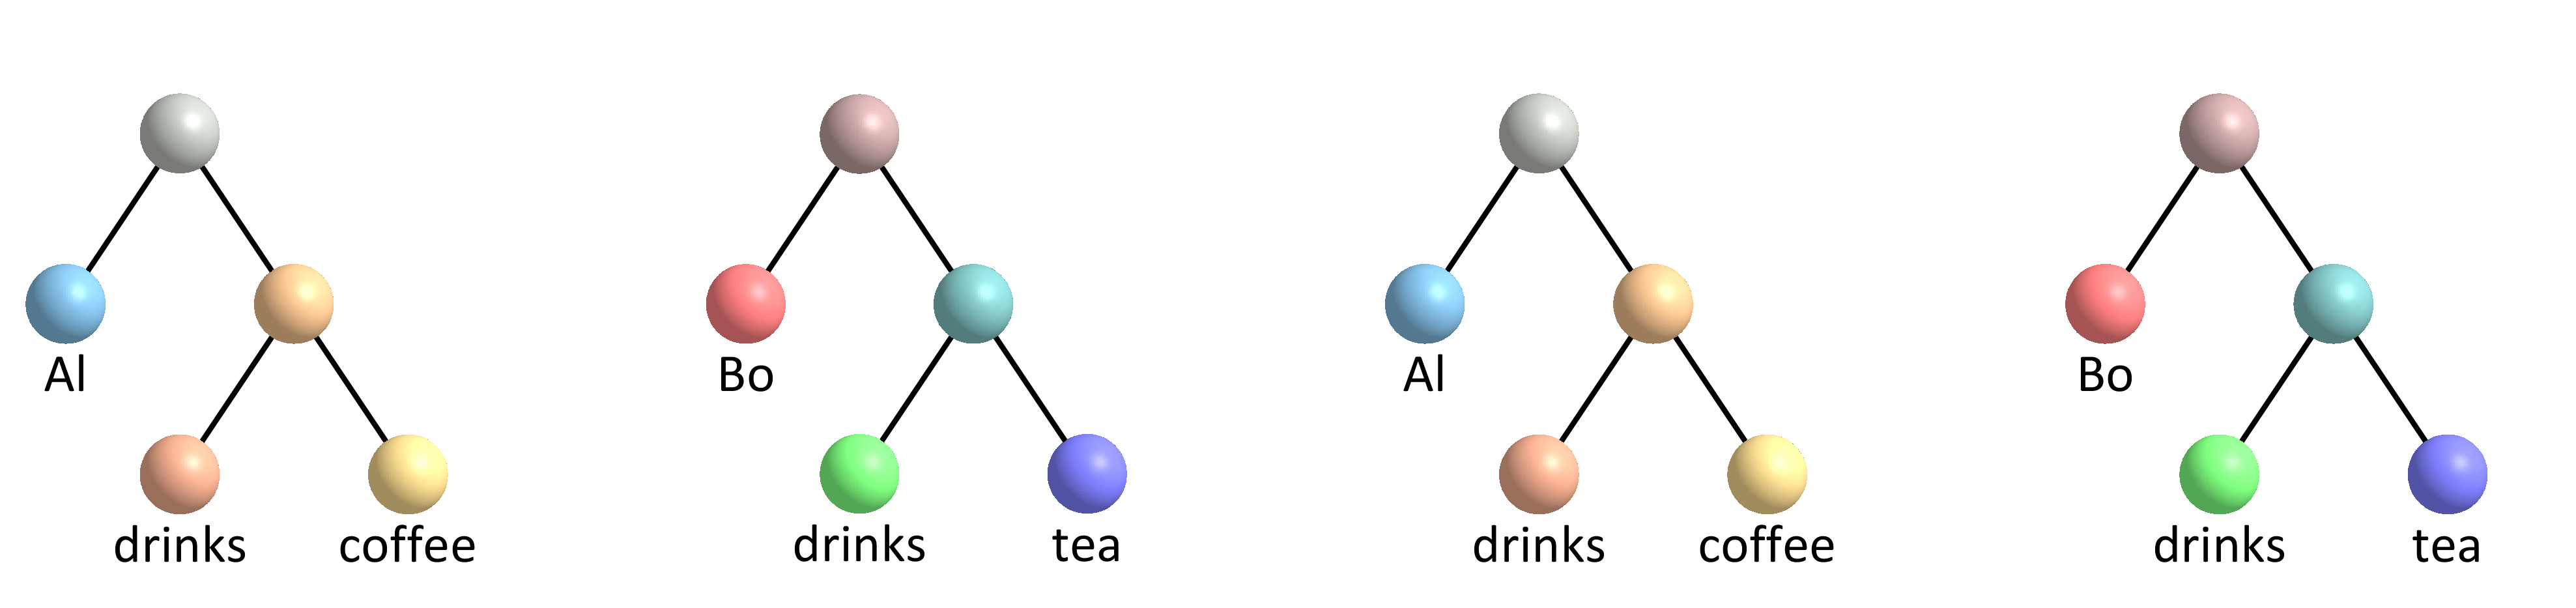
\includegraphics[width=\textwidth]{figures/Tilsen-img8.png}
\caption{\missingcaption}
\label{fig:}
\end{figure}
 

  Are schemas of this sort useful? Imagine the following scenario, in which you engage two thought patterns in succession. First, you engage the pattern \textit{Al drinks coffee}. Next, you engage an alternative pattern, \textit{Bo drinks tea}. Then, you return your attention to \textit{Al drinks coffee.} Then, back again to \textit{Bo drinks tea}. And so on… What would we expect to observe in the brain in this scenario? 

  The connected objects schema is not well suited for addressing this question. Because these sentences are conceptualized as structures of objects, we can ask: “where do the objects come from?”, “how do they become connected or combined?”, and “what happens to them when we switch to a different pattern?” Do the objects get destroyed? Do they move somewhere? Do they vanish, are they hidden? Do the objects ever change over time? Where are these objects located in space? Etc.

  The essence of the problem is that conventional approaches force us to think of linguistic units \textit{as objects}. To construct abstract understandings of phenomena, we often use the \textsc{abstractions-}\textsc{are}\textsc{{}-objects} metaphor (e.g. \textit{put your feelings aside}, \textit{tear an argument into pieces}, \textit{build a new life}, etc.). But regardless of how familiar it is and how intuitive it seems, the \textsc{units}\textsc{{}-are-}\textsc{objects} metaphor is not necessarily a useful conceptualization of language. 

  In the o/el framework, linguistic units are \textit{not} objects. They are not the sorts of things that contain meaning, and are not the sorts of things that can be connected. They do not occupy space, they do not have orientational relations. The o/el framework rejects all entailments of the \textsc{units}\textsc{{}-are-}\textsc{objects} metaphor. Instead, we adopt an alternative in which meanings are experiences, experiences are trajectories of system states in a state space, and various forces influences those trajectories. Our task then becomes construction of a state space, analysis of state trajectories, and determination of forces. Because meaning experiences are trajectories, meanings are inherently temporal. 

\subsection{Concept-specific populations of neurons}

To develop an intuition for the \textsc{meanings}\textsc{{}-are-}\textsc{trajectories} metaphor we consider a simple utterance, \textit{Al drinks coffee.} We pose the following question: \textit{physically}, in space and in time, what happens when a speaker produces this utterance? Lets suppose that in some brief period of time preceding the utterance, in the brain of the speaker, there is a population of excitatory cortical neurons which in a statistical sense\footnote{To assess this empirically, we would want high-spatial and temporal resolution of electrochemical gradients and synaptic connectivities, along with information regarding movements and acoustic signals. Whether this can be accomplished with current technology is beside the point: we can imagine associating populations of neurons with concepts in this way. Note that we require no assumptions about the uniqueness or overlap of the populations at this point. The idea that spiking in distributed populations of neurons (or assemblies, ensembles, etc.) may correspond to things like concepts or words is a fairly old one; see for example (\citealt{Abeles2012,Braitenberg1978,Hebb1949}; Pulvermüller, 1999)} is associated with concepts that contribute to the relevant experience of meaning. For exposition, lets identify those concepts as [Al], [drinks], and [coffee]. Furthermore, suppose that we can differentiate the population into an [Al] subpopulation, a [drinks] subpopulation, and a [coffee] subpopulation. Thus each concept is associated with a population of many neurons. No strong assumptions are necessary regarding the temporal permanence, spatial distributions, sizes, or independence of these concept populations.

  
\begin{figure}
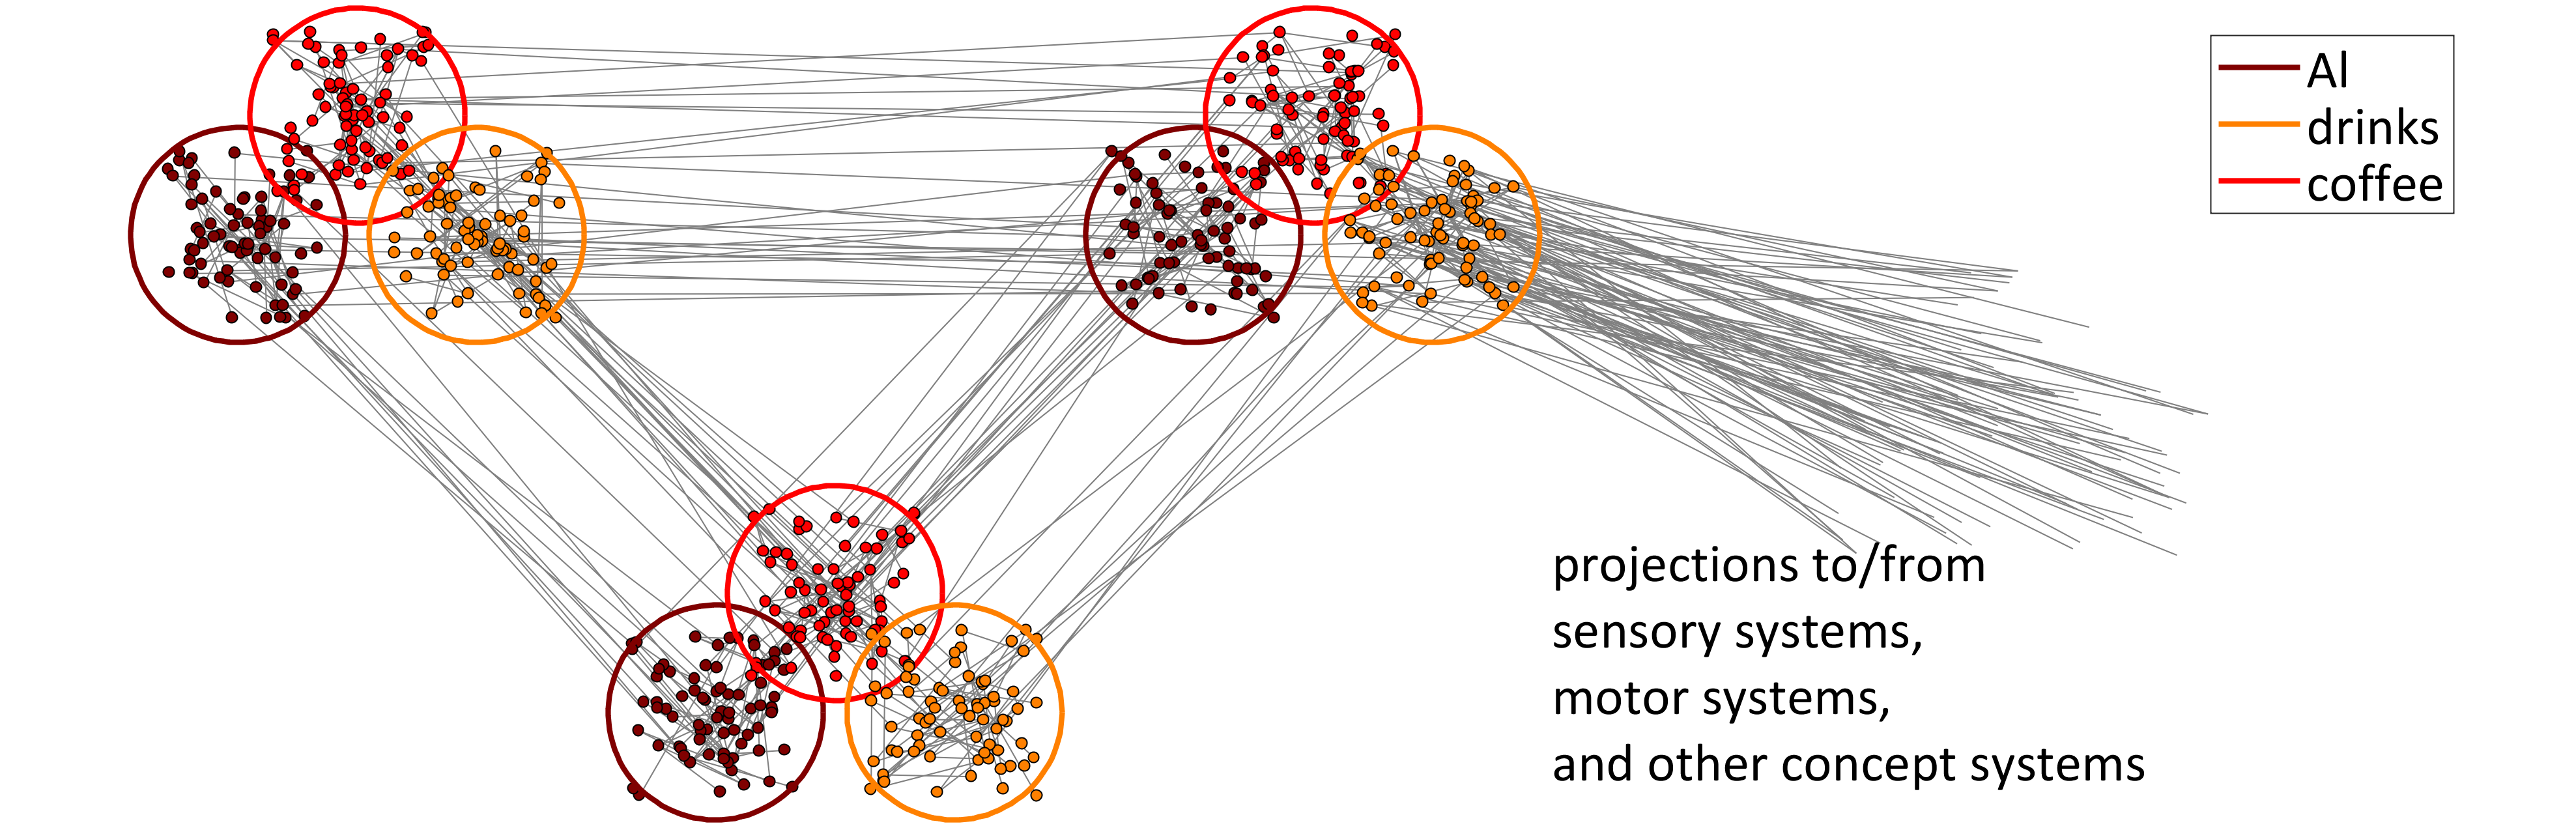
\includegraphics[width=\textwidth]{figures/Tilsen-img9.png}
\caption{\missingcaption}
\label{fig:}
\end{figure}
 

  The picture above shows populations that are \textit{distributed}: concept populations are associated with neurons in multiple regions of the brain, rather than just one region. Moreover, the “meanings” of concepts are qualia which we assume to be determined by the structure of projections to and from sensory systems, motor systems, and other concept populations. For example, our experience of \textsc{coffeeness} is a consequence of patterns of projections to and from the peripheral sensory systems which provide us information regarding taste, odor, appearance, temperature, etc. of coffee, as well as the motor systems which we use to pour coffee, drink it, brew it, and also other concepts which relate to \textit{coffee}: beans, cups, caffeine, etc. There is no essential meaning of \textit{coffee} because the pattern of projections varies over time within an individual and varies in space, i.e. between individuals.
\subsection{{\textbf{Phase transitions to collective oscillation}}}

Before a speaker experiences a meaning associated with [Al], [drink], and [coffee], the neurons of each of these concept populations must undergo a phase transition from an \textit{inactive} regime, in which action potentials are sparse in time and relatively uncorrelated, to an \textit{active} regime, in which action potentials are frequent and highly correlated. We conjecture that integrating action potentials for each population on an appropriate timescale results in an oscillatory spike-rate\footnote{There is plenty of evidence that oscillation plays an important role in the nervous system, and that neural populations exhibit oscillatory patterns of spiking (\citealt{AverbeckEtAl2003,Buzsaki2006,BuzsákiDraguhn2004,CanoltyKnight2010,EngelEtAl2001,Fuster2001,GerstnerKistler2002,Izhikevich2006,Izhikevich2007,IzhikevichEdelman2008,Klimesch1999}). However, because concept populations are hypothetical, the assumption that these populations oscillate is a conjecture.}, as shown below. We conceptualize this phenomenon as the emergence of a macroscopic \textit{collective oscillation} \citep{AcebrónEtAl2005,BreakspearEtAl2010,HongStrogatz2011,Kelso1997,SchonerKelso1988,Strogatz2000,Winfree2001}. The causes of these phase transitions are various, but lets imagine for concreteness that the speaker sees a man named \textit{Al} and a dark liquid falling into his mouth from a cup he holds. We infer that this peripheral sensory information, through a chain of interactions, causes the relevant concept populations to undergo transitions to the collective oscillation regime.


  
\begin{figure}
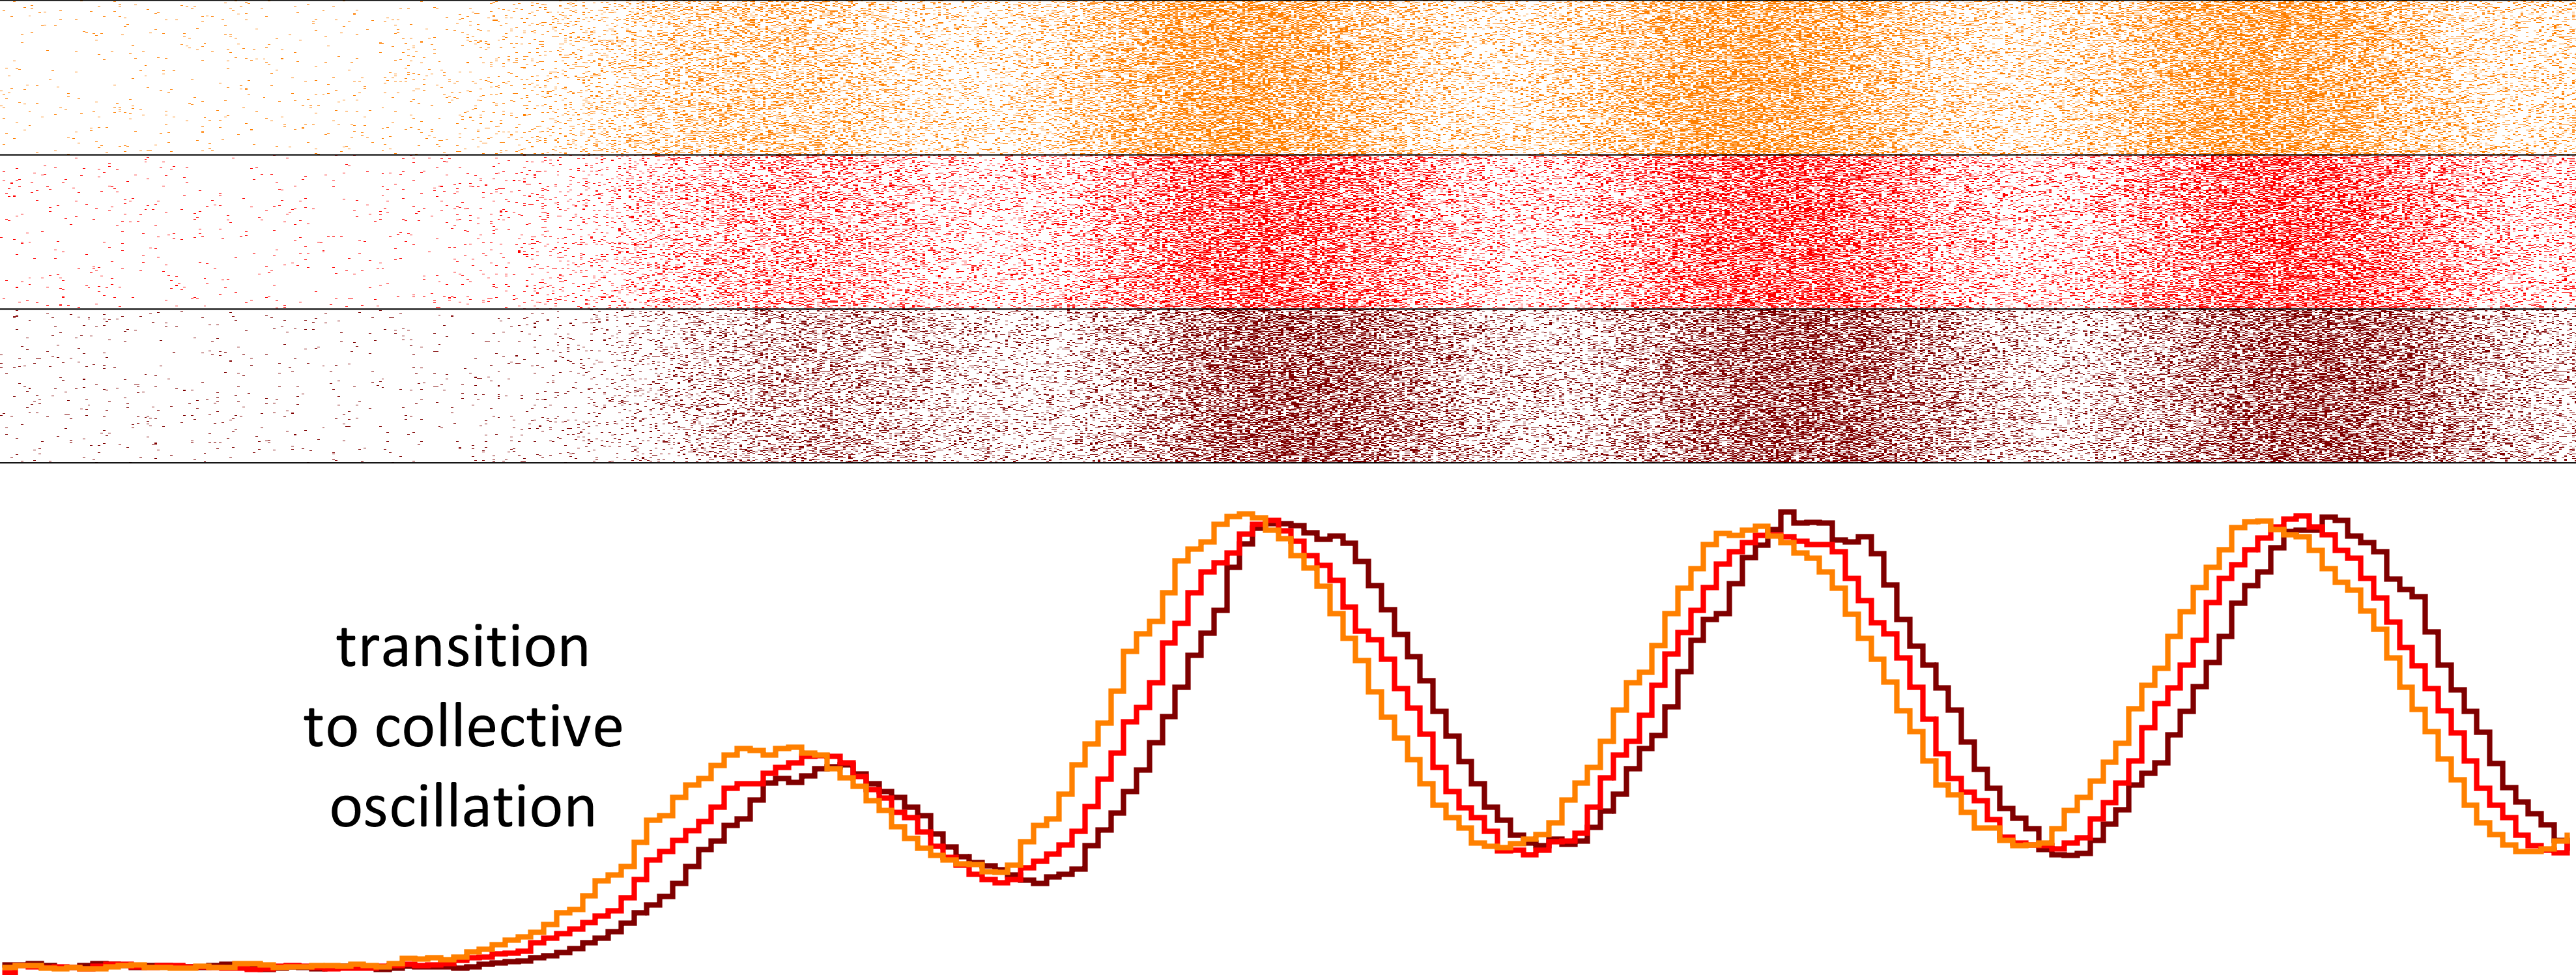
\includegraphics[width=\textwidth]{figures/Tilsen-img10.png}
\caption{\missingcaption}
\label{fig:}
\end{figure}
 

  The transition to collective oscillation is a localized emergence of a state that is highly ordered in space and time. The microscopic state space has many dimensions. There are numerous degrees of freedom: membrane voltages, ion channel states, neurotransmitter concentrations, etc., of all of the neurons in the relevant populations. In contrast, the macroscopic pattern of oscillation, which we obtain by integrating strategically over the microscopic variables, represents a drastic reduction in the volume of this state space, and is far more practical as an analytic tool. The transient oscillations have only several degrees of freedom: phase angle (θ), angular velocity ($\theta ′$) i.e. instantaneous frequency, and radial amplitude (\textit{r}).

\subsection{{\textbf{Concept populations as systems with surroundings}}} 

To be explicit, we model each concept population as a \textit{concept system} with a time-varying state vector. Interactions between systems are forces, which depend on system states. Moreover, each system has a surroundings. These constructs—\textit{systems}, \textit{states}, \textit{forces}, and \textit{surroundings}—are derived from our microscopic population model. Systems are macro-scale models of populations. System states derive from integrating over population microstates. Forces between systems derive from integrating over the influences of synaptic projections from neurons in one population to another. The surroundings derives from integrating microscale influences, the origins of which we do not differentiate as systems.\footnote{The surroundings is where we locate our ignorance in a given analysis. We can always improve our analyses by constructing new systems from the surroundings, but so doing, the analysis becomes more complex. We often to refer to the influence of the surroundings, and this should be viewed as consequence of oversimplification.} These constructs are illustrated below.

  
\begin{figure}
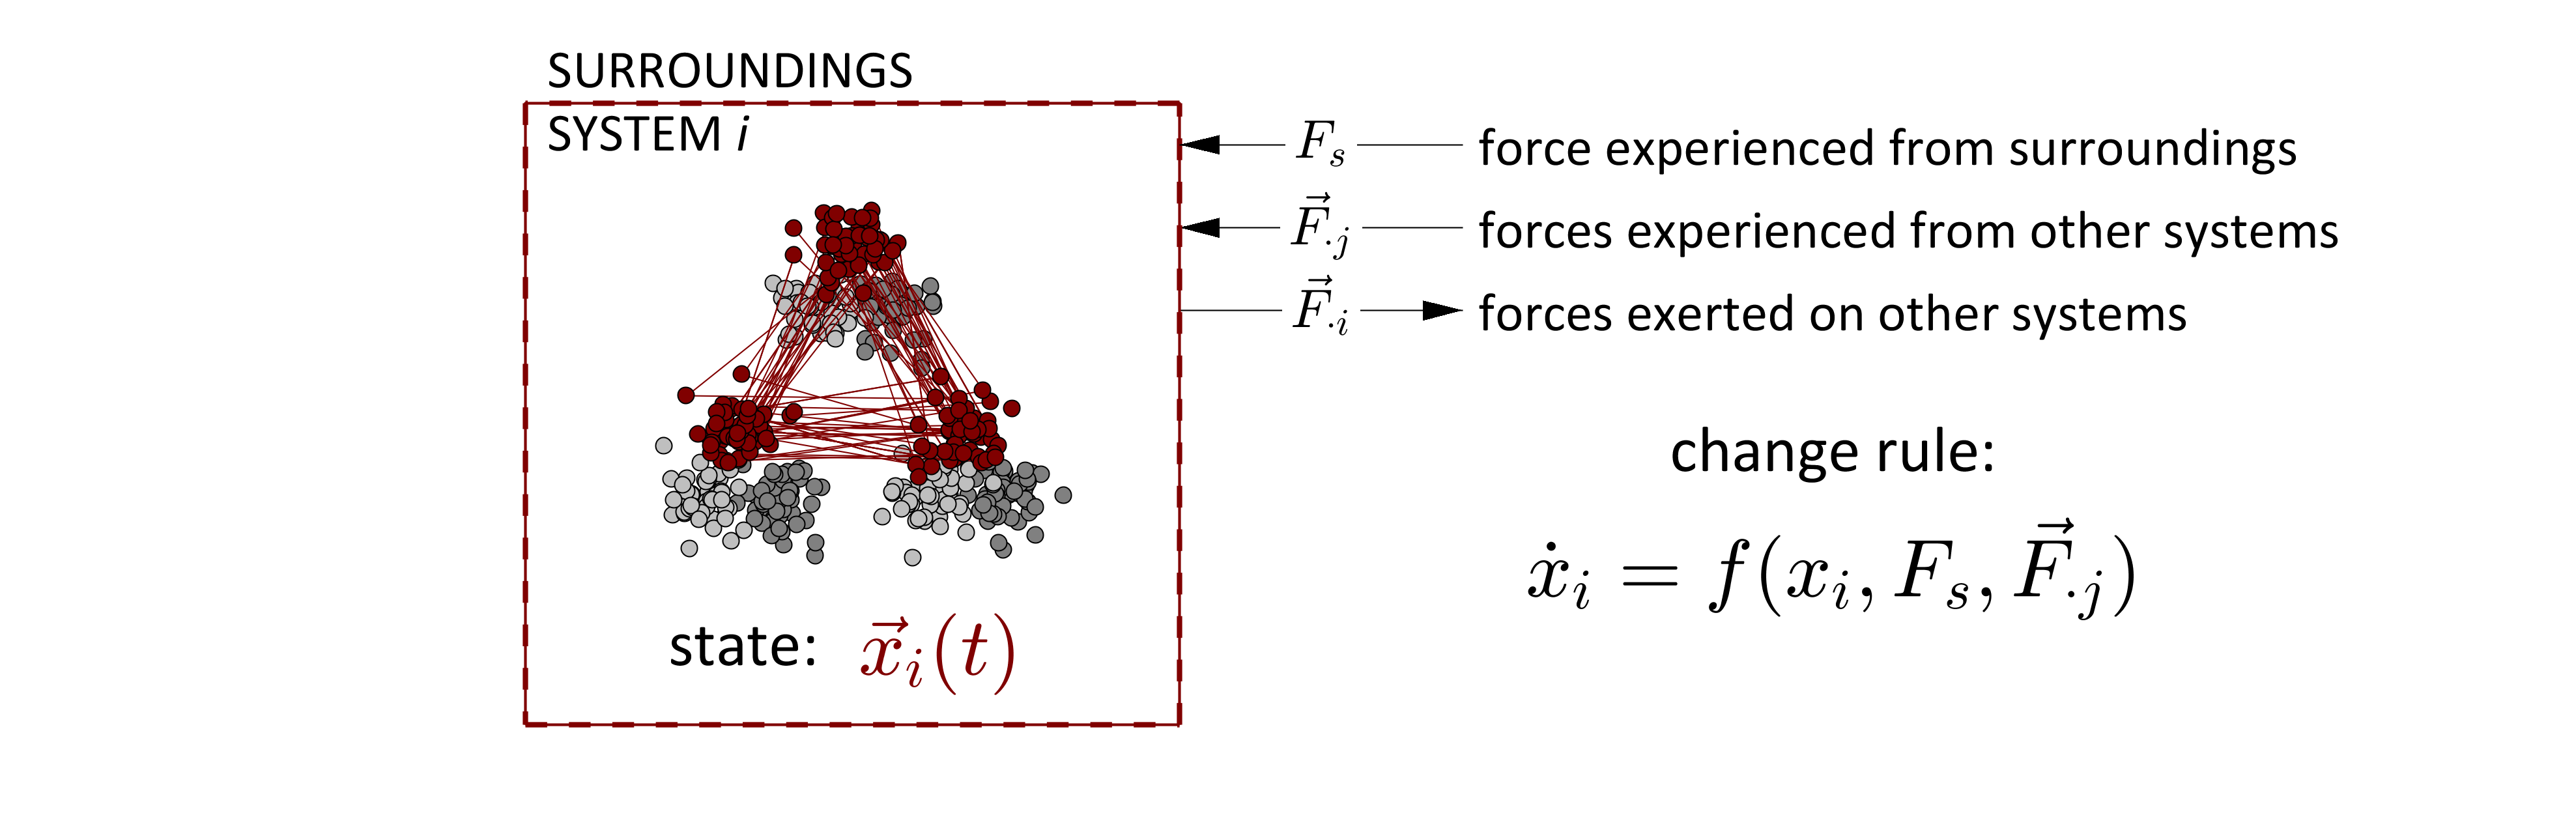
\includegraphics[width=\textwidth]{figures/Tilsen-img11.png}
\caption{\missingcaption}
\label{fig:}
\end{figure}
 

\subsection{System state variables: excitation and phase}

To construct a change rule for system states, we must define the state space. To do this, we reconceptualize the spike-rate of each population, i.e. a time-integration of action potentials, as a macroscopic \textit{order parameter}, \textit{A}. The order parameter \textit{A} is the deviation of the spike rate from a reference value associated with the inactive regime. Furthermore, we conjecture that when a system activates, variation in the order parameter has two components: an oscillation component x\textsubscript{osc}, and an excitation component x\textsubscript{exc}, whose sum is the order parameter, i.e. \textit{A} = x\textsubscript{osc} + x\textsubscript{exc}. We then approximate the oscillation component as a harmonic oscillation with time-varying amplitude and phase angle, i.e. x\textsubscript{osc} = r(t) cos θ(t).The phase variable θ of a system is taken to be 2π{}-periodic, evolves according to an intrinsic system frequency \textit{f}\textsubscript{0}, and is influenced by forces from other systems and the surroundings. The radial amplitude of x\textsubscript{osc} is assumed to be proportional to the excitation component of the system, i.e. r  ${\propto}$ x\textsubscript{exc}. This analysis of \textit{A} is schematized below.  

  
\begin{figure}
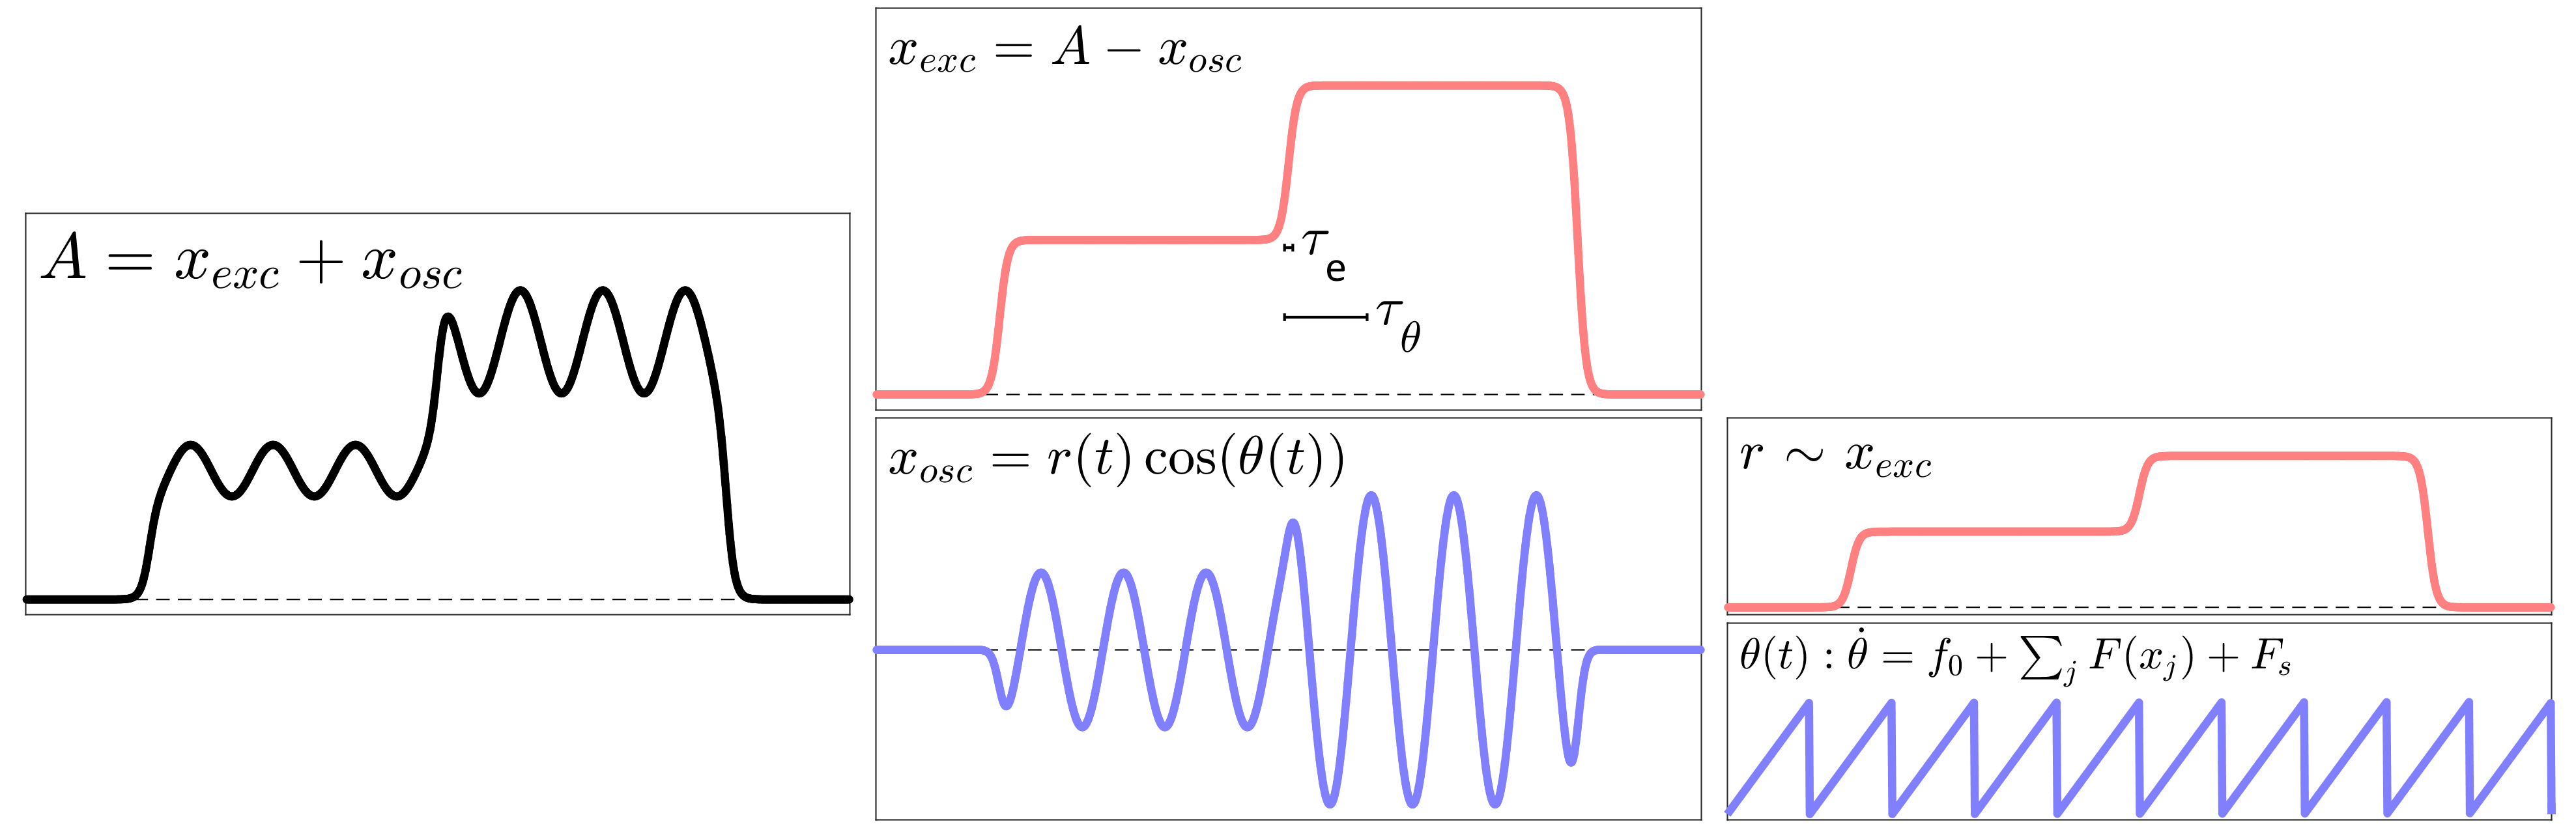
\includegraphics[width=\textwidth]{figures/Tilsen-img12.png}
\caption{\missingcaption}
\label{fig:}
\end{figure}
 

  For exposition, we rename the excitation component x\textsubscript{exc} as (\textit{e}) and refer to phase angle (θ) simply as \textit{phase}. We make a heuristic simplification by assuming the dynamics of \textit{e} and θ are separable due to differences in relevant timescales. This stipulated separation entails that there is a fast timescale τ\textsubscript{e} such that changes in \textit{e} occur over intervals τ\textsubscript{e}, and τ\textsubscript{e} << τ\textsubscript{θ} = 1/\textit{f}, the period of the oscillation. Hence in our analyses of the dynamics of \textit{e} and θ, intermittent abrupt changes in \textit{e} are assumed not to interact directly with θ. Furthermore, the intrinsic frequency \textit{f}\textsubscript{0} is considered to be slowly-varying on utterance timescales, and for some purposes can be conceptualized as a fixed parameter. 

  Given the above construction, the state space for one concept system is the union of subspaces for \textit{e} and θ. We do not attempt to provide a more detailed derivation of these variables and their separation from a microscopic, population-scale model. Nonetheless, we speculate that oscillation arises from intra-population synaptic interactions, intrinsic neuronal dynamics, cortical microcircuit structure, and coupling between neurons and the extracellular medium, whereas excitation relates more directly to the number of neurons which participate in a population oscillation.  

\subsection{Meaning experiences are trajectories in state space}

The utterance \textit{Al drinks coffee} does not “have” a meaning. An utterance can only \textit{have} a meaning if we presuppose that meanings are objects contained in words. We reject these object and containment metaphors. Instead, meanings are experiences which correspond to trajectories in concept system \textit{e},θ space. The conventional object and o/el trajectory metaphors are contrasted below. In o/el terms, a meaning experience associated with a single concept arises when two conditions are met: (i) a stable periodic trajectory occurs in the θ subspace associated with a concept, for an interval of time on the order of τ\textsubscript{θ}, and (ii) the excitation of the concept exceeds a threshold value λ\textsubscript{e}. When \textit{e} > λ\textsubscript{e} we refer to the system as \textit{excited}; when 0 < \textit{e} < λ\textsubscript{e}, we refer to the system as \textit{active}; when e = 0 we refer to the system as \textit{inactive}. The phase θ of an inactive system is undefined, because by definition the inactive state entails no collective oscillation. 

  
\begin{figure}
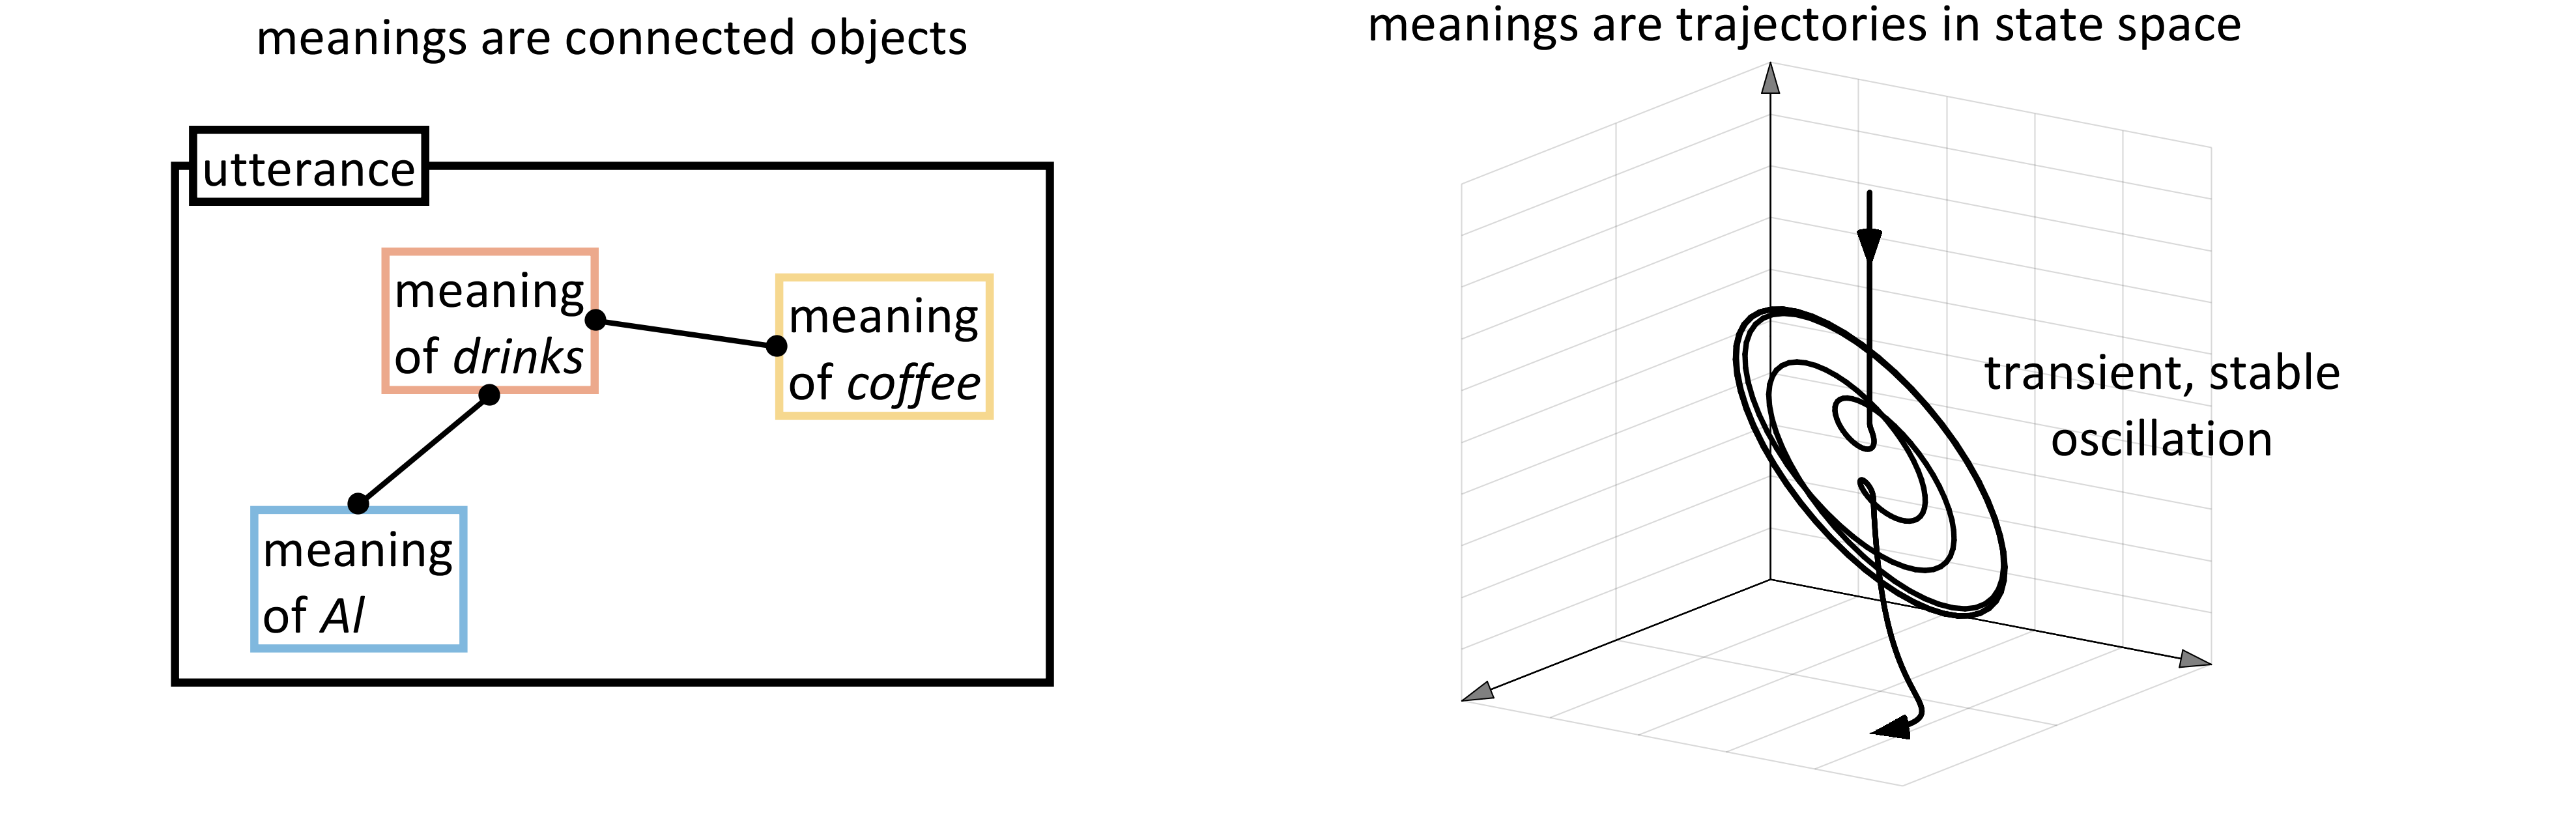
\includegraphics[width=\textwidth]{figures/Tilsen-img13.png}
\caption{\missingcaption}
\label{fig:}
\end{figure}
 

  The \textit{e},θ state space is 2-dimensional for one concept system, and 2\textit{n}{}-dimensional for \textit{n} concept systems. Moreover, when \textit{n} concept systems are excited, a relational meaning experience associated with those systems is a stable periodic orbit in the \textit{n}{}-dimensional θ subspace. Typically we are interested in meaning experiences associated with systems whose \textit{e} > λ\textsubscript{e}, i.e. excited systems. We will sometimes refer to these as \textit{attended} meanings, because we imagine that the relevant concept systems have \textit{e} values which are sufficient to support conscious attention to a meaning experience. In contrast, subconscious experience of meaning occurs via active, unexcited systems.

  Note that \textit{e} and θ state variables are analytical constructs which we can attempt to derive from a higher-dimensional microscale state space. This derivation procedure uses methods of projection and integration in order to reduce dimensionality. Accordingly, the state space is always constructed \textit{ad hoc} to accommodate the systems which we consider relevant for a given analysis. The state space construction procedure is (i) stipulate concept systems; (ii) construct a space with \textit{e} and θ dimensions for each system; (iii) construct the union of these spaces by combining them orthogonally. The picture to have in mind is below. 

  
\begin{figure}
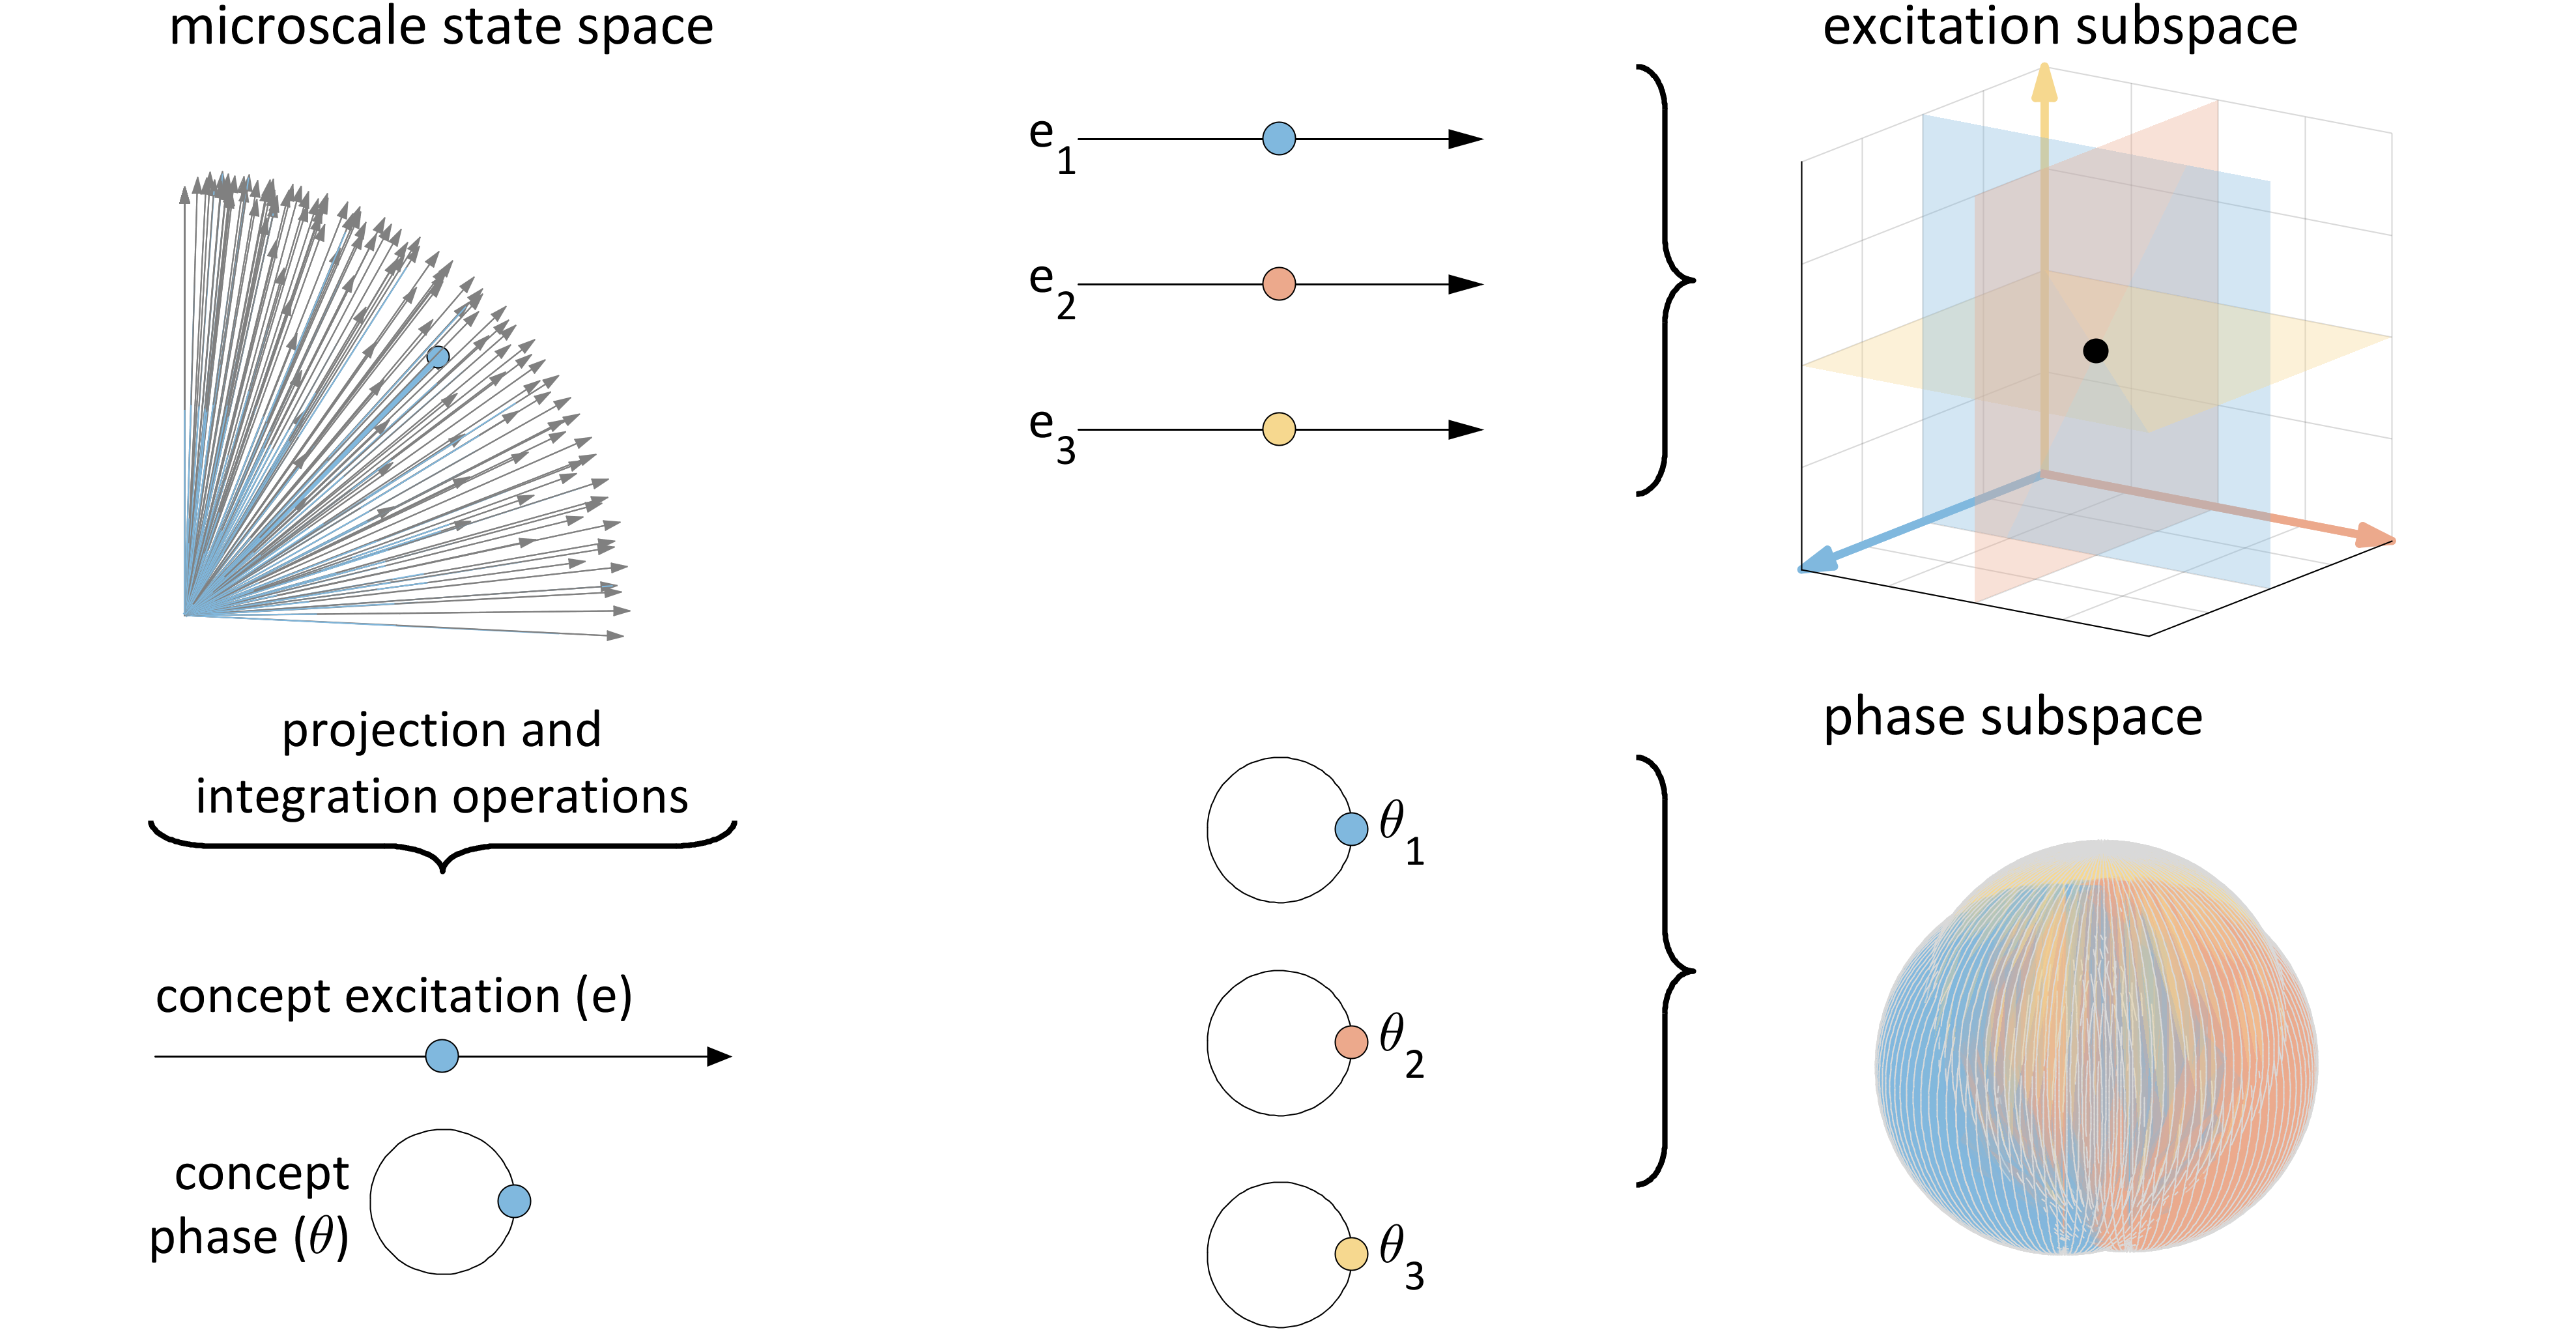
\includegraphics[width=\textwidth]{figures/Tilsen-img14.png}
\caption{\missingcaption}
\label{fig:}
\end{figure}
 

  The state space is neither permanent nor a physical space. It is a heuristic tool that we construct strategically to meet the needs of a given analysis. Describing [Al], [drinks], and [coffee] with orthogonal excitation and phase variables is useful because it provides a coarse model of the much higher-dimensional states of neural populations. Conceptualizing meaning experiences as trajectories in the e,θ space opens up a new approach to reasoning about linguistic phenomena.

\subsection{Relational meaning experiences are relative phase configurations}

Individual concept meaning experiences rarely occur in isolation. The production of \textit{Al drinks coffee} is associated with simultaneous excitation of concepts [Al], [drinks], and [coffee]. Yet simultaneity of excitation is not sufficient for understanding the \textit{relational} character of meaning experiences. This is obvious from consideration of utterances such as \textit{Al likes Bo} and \textit{Bo likes Al}, where the same concepts are excited and yet different relational meanings are experienced. Since we do not experience both of these relational meanings simultaneously, there must be a mechanism which distinguishes system states in which [Al] and [Bo] have different relations to [likes]. Moreover, this mechanism should also govern the relations of [Al] and [coffee] to [drinks] in \textit{Al drinks coffee}, as well as any arbitrary relations of this sort. 

  To that end we propose a \textit{principle of relational meaning}: relational meaning experiences are stable relative phase configurations. Recall that relative phase φ is defined as the antisymmetric difference of phases, i.e. φ\textsubscript{ij} = θ\textsubscript{i} - θ\textsubscript{j} = -φ\textsubscript{ji}. For exposition we often refer to φ without indices and interpret this as the absolute value of relative phase, i.e. {\textbar}φ{\textbar} = {\textbar}θ\textsubscript{i} – θ\textsubscript{j}{\textbar}. Furthermore, we pursue a strong hypothesis that all relational meaning experiences are associated with a stable states in which φ ${\approx}$ 0 or π, which we call \textit{in-phase} and \textit{anti-phase}, or \textit{proximal} and \textit{distal} φ configurations, respectively. More precisely, for any pair of concept systems \textit{i} and \textit{j}, a relational meaning experience occurs when both systems are excited \{e\textsubscript{i}, e\textsubscript{j}\} > λ\textsubscript{e} and have a stable relative phase such that {\textbar}φ\textsubscript{ij}{\textbar} ${\approx}$ \{0, π\} and dφ\textsubscript{ij}/dt ${\approx}$ 0. Specifically, we hypothesize that in-phase states (φ ${\approx}$ 0) are associated with agent-action relations, e.g. [Al][drinks], and that anti-phase states (φ ${\approx}$ π) are associated with patient-action relations, e.g. [drinks][coffee]. These are summarized in the {\tablebelow}. Many additional φ-relation hypotheses are developed subsequently.

  \begin{table}
\begin{tabularx}{\textwidth}{XXll}
  \lsptoprule
  \multicolumn{2}{c}{\textbf{conceptual systems}} & 
  \textbf{semantic relations} & 
  \textbf{$\varphi$ configurations}\\
  \midrule{}
  [Al] & [drink] & agent-action & in-phase: φ ${\approx}$ 0\\{}
  [coffee] & [drink] & patient-action & anti-phase: φ ${\approx}$ π\\
  \lspbottomrule
  \end{tabularx}
\caption{\missingcaption}
\label{tab:key:}
\end{table}

  The φ configurational basis for differences in relational meaning between [Al][drinks] and [coffee][drinks] is illustrated below. Crucially, [Al][drinks] and [coffee][drinks] φ configurations remain constant despite the fact that all three θ variables are changing. Constant φ, when stable over time periods on the order of τ\textsubscript{θ}, gives rise to the experience of relational meaning between systems, as long as those systems are excited. Note that φ configurations are periodic trajectories in θ space, but we can also construct a φ space in which a stable φ configuration is a point. Moreover, because θ dimensions are circular, wrapping around the interval [0, 2π], φ patterns can also be represented as a static phase difference on a unit circle, as below. In such representations we choose some system as a reference, and the phase angles of all other systems are shown relative to the phase of the reference system. For visual clarity, we depict systems with a φ=0 configuration as having a small φ separation, as with [Al] and [drinks] below.

  
\begin{figure}
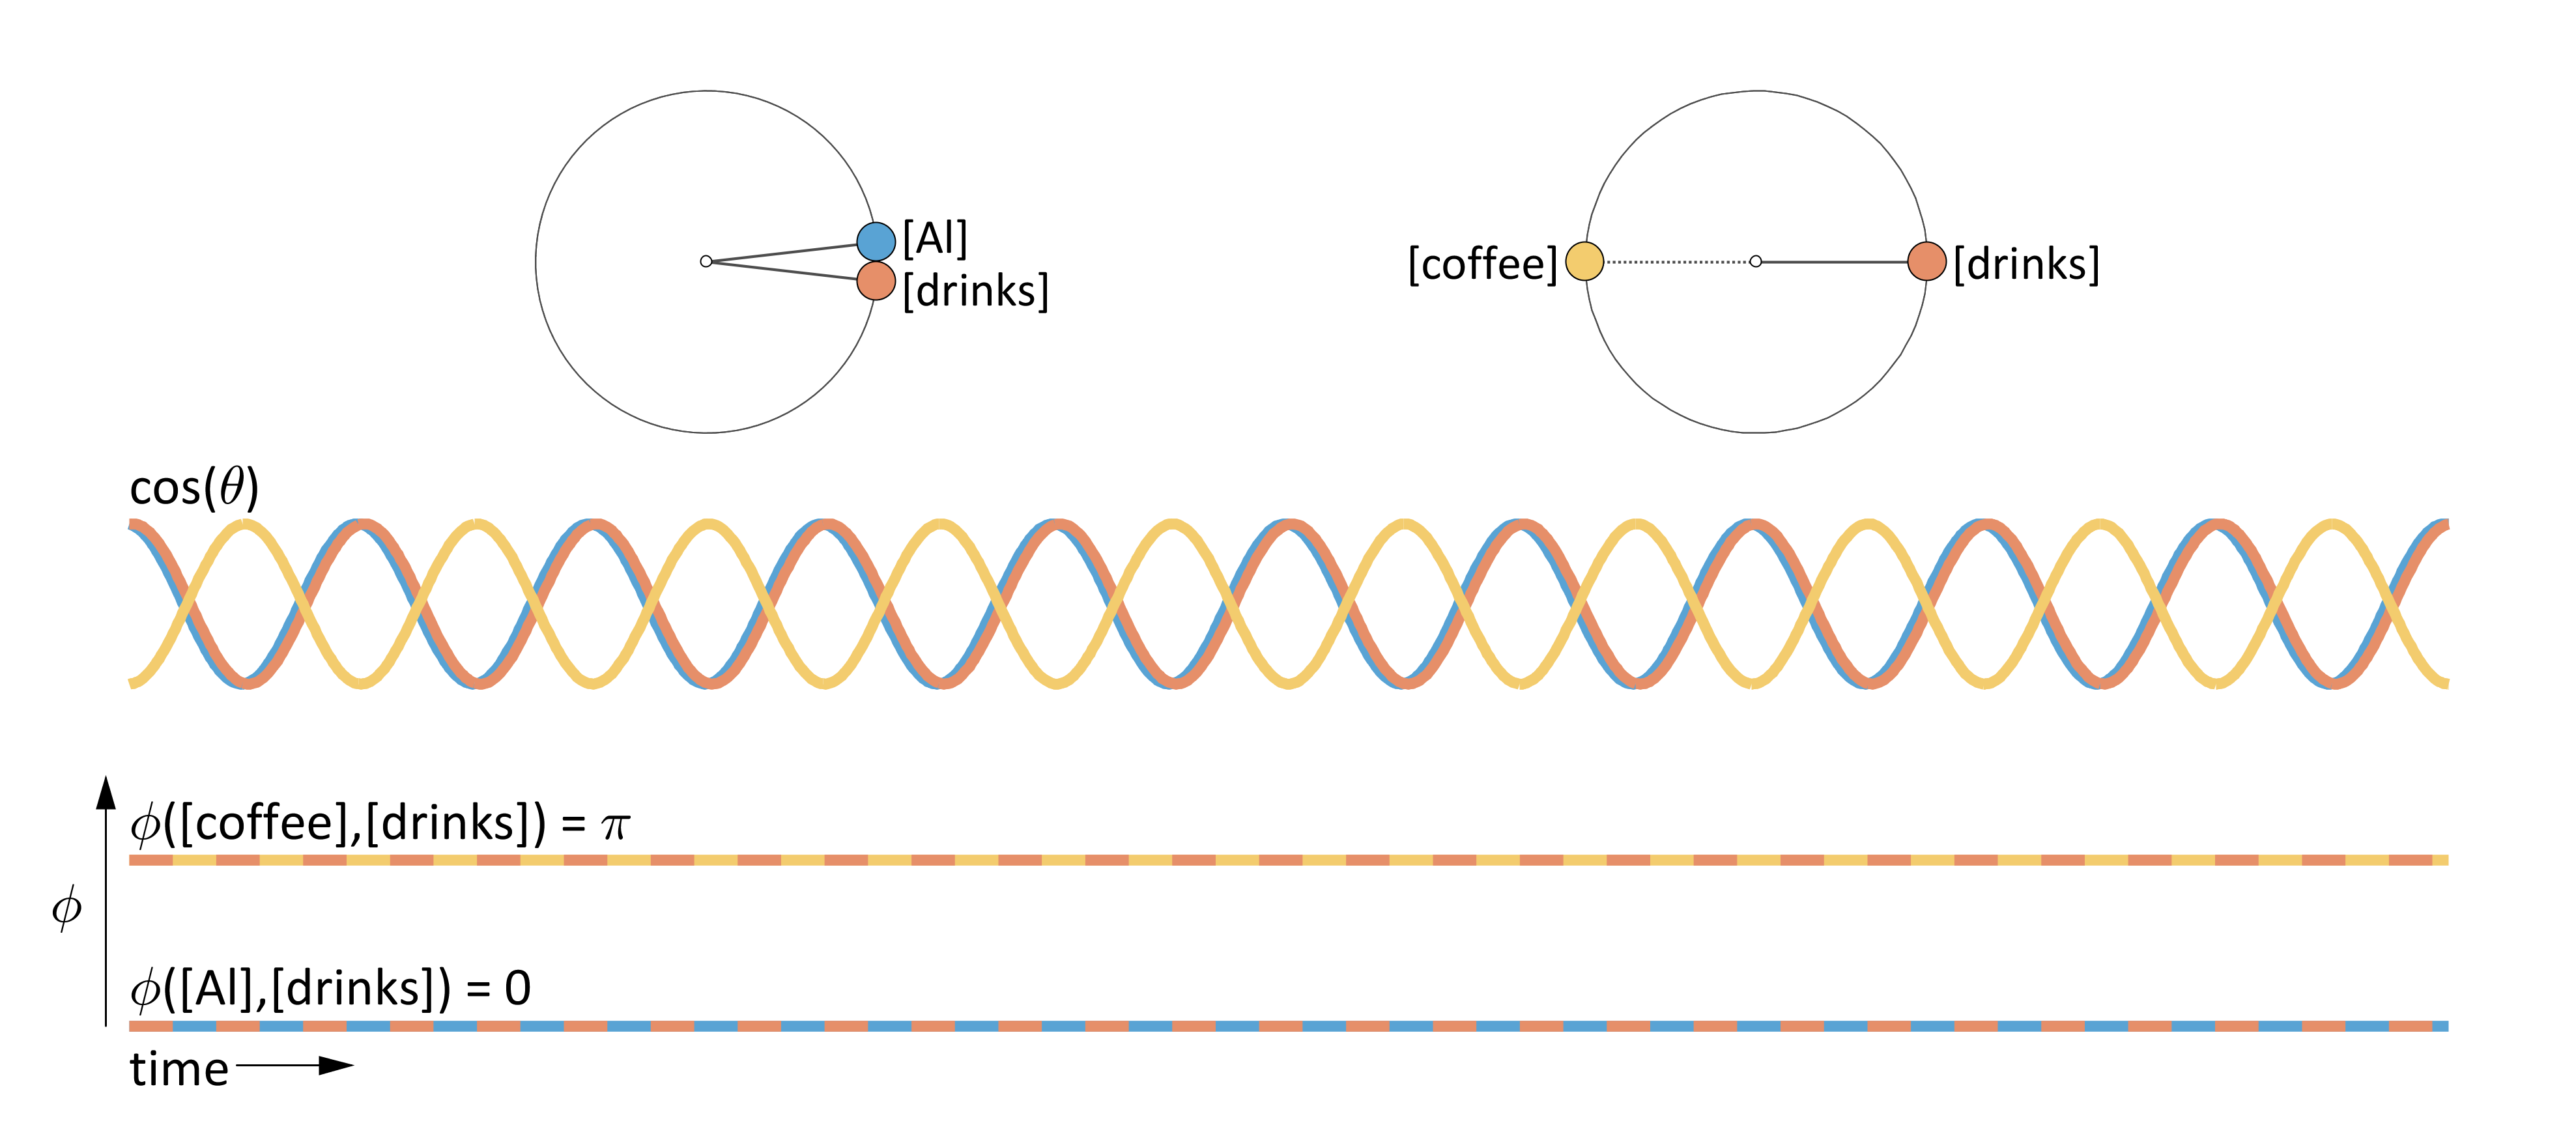
\includegraphics[width=\textwidth]{figures/Tilsen-img15.png}
\caption{\missingcaption}
\label{fig:}
\end{figure}
 

  The principle of relational meaning requires relational meaning experiences to be \textit{stable} φ configurations. Here \textit{stable} means that φ, when perturbed, returns to an equilibrium value (0 or π) on a timescale which is substantially less than τ\textsubscript{θ}. Fluctuations constantly perturb θ variables of systems and hence perturb φ. A stabilizing mechanism is thus required to force φ back an equilibrium value. 

  What is the stabilizing mechanism? Our microscopic model suggests that synaptic projections between concept systems and other systems could accomplish this stabilization. By integrating over interpopulation synaptic projections we can derive macroscopic \textit{coupling forces}, which serve to stabilize φ. However, if these forces act directly between concept systems, there is a problem…

\subsection{Direct interactions between conceptual systems are unlearnable and inflexible.} 

Lets imagine that a direct interaction between [Al] and [drinks] concept systems were indeed responsible for stabilizing their φ configuration. On the basis of our microscale conception, such interactions must be learned: macroscopic forces are derived from synaptic weights (i.e. efficacy of neurotransmitter release/uptake), connectivity patterns, etc. between populations. Learning is an evolution of these variables on supra-utterance timescales. Moreover, the interaction, if a stabilizing one, would need to be fairly strong, otherwise moderate perturbations would overcome the equilibration forces. 

  There are two problems with the direct coupling scenario. The first involves learnability. Two different types of interactions between [Al] and [drinks] would need to be learned, i.e. an in-phase and anti-phase interaction for the agent and patient roles, respectively. Moreover, these two types of interaction would need to be learned for all \textit{pairs} of concepts: for \textit{n} concept systems there are 2\textit{n}\textsuperscript{2} interactions. The second problem involves flexibility. If the learned stabilizing interactions are too strong, then there is a danger that excitation of one concept system will always cause other concept systems that it interacts with to become excited. For example, imagine that when [Al] becomes excited, direct interaction forces excite [drinks] and [coffee] as well. This is a problem if one wants to experience the meaning of \textit{Al eats granola}, for example. With direct interactions between concept systems, system trajectories would be prone to seizures in which all concept systems become excited. The solutions to the flexibility and learnability problems are provided by syntactic systems.

\section{Syntactic systems}

Syntactic systems are the primary mechanism for stabilizing φ configurations of concept systems. There are two basic aspects of this mechanism. First, concept systems resonate with syntactic systems through mutual positive feedback. We refer to this as \textit{resonance} because syntactic systems have strong, asymmetric interactions with concept systems. Second, syntactic systems couple strongly to other syntactic systems. Hence syntactic systems can organize and stabilize φ configurations between concept systems, without requiring strong direct coupling between concept systems. Syntactic systems provide an \textit{indirect}, \textit{flexible} mechanism for stabilizing relational meaning, one which does not rely on learning direct interactions between concepts. Henceforth we abbreviate concept systems as \textit{c-systems}, and syntactic systems as \textit{s-systems}. 

\subsection{Microscopic conception of syntactic and conceptual systems}

Both s- and c-systems have \textit{e} and θ state variables, and these are derived in the same way from a microscale conceptualization of populations. But the microscopic pictures of c-systems and s-systems differ in some important ways which help resolve the learnability and flexibility problems. First, for concepts we imagine a large, distributed population of neurons. Each individual c-system is a subpopulation of this full population, and despite substantial overlap of these subpopulations, c-systems can be distinguished from each other on the basis of their interactions with other systems and the sensorimotor surroundings. On the macroscale, the primary mechanism of learning is not “adding” new c-systems, but rather differentiating and blending existing c-systems. On the microscale this entails that new sub-populations are not “created”, but rather new patterns of interaction arise with the sensorimotor surroundings and other conceptual systems. Interactions between c-systems are presumed to be relatively weak: c-systems can activate other c-systems (this is often called \textit{priming}), but typically do not excite other c-systems.

  
\begin{figure}
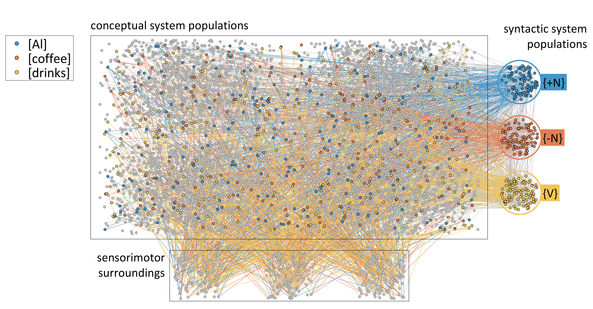
\includegraphics[width=\textwidth]{figures/Tilsen-img16.png}
\caption{\missingcaption}
\label{fig:}
\end{figure}
 

  In contrast to the full population of c-systems, the full population of s-systems is spatially localized, possibly in the inferior frontal gyrus. Individual s-systems, i.e. subpopulations of the full s-system population, overlap to lesser degree with each other than c-systems do, and interact more strongly because of their spatial localization. 

  The c- and s-system populations project to one another, and under certain conditions c-system populations may resonate with s-system populations, a phenomena we refer to as \textit{cs-resonance}. We assume that the capability for cs-resonance is phylogenetic, but in development, different c-systems become preferentially biased to resonate with different types of s-systems. Furthermore, we speculate that the effects of general learning mechanisms (e.g. Hebbian spike-timing dependent synaptic plasticity), when integrated on supra-utterance timescales, differentiate the full syntactic population into various s-system subpopulations. Biases for in-phase and anti-phase coupling interactions between s-system populations are learned in this manner, giving rise to a grammar of φ coupling. A more thorough discussion of learning in the o/el framework is undertaken later on, but the primary focus of this book is the analysis of utterance-timescale patterns in speech.

\subsection{Conceptual systems resonate with syntactic systems}

The cs-resonance mechanism can be understood as follows. First, forces from the surroundings activate a c-system and a corresponding s-system. These systems begin to resonate weakly, in a positive mutual feedback interaction. Microscopically, the positive feedback resonance mechanism derives from integrating the effects of excitatory-to-excitatory interpopulation projections between an s-system and c-system. Because these projections are excitatory, resonating c- and s-systems always have an in-phase φ-relation. 

  Recall that activation implies a collective oscillation, but not stability of θ′ and not necessarily an \textit{e} value sufficient for a meaning experience. In general many c-systems may be active and may compete for resonance with a given s-system; surroundings forces influence this competition as well. The competition from other c-systems and surroundings forces can potentially destabilize a newly formed resonance between c- and s-systems. We thus imagine a pre-stable phase of production in which interaction between a c- and s-system may or may not lead to a strong cs-resonance. If positive feedback between the c- and s-system is sufficiently strong relative to destabilizing forces, the c- and s- system abruptly become \textit{excited}, which entails that the s-system \textit{e} value exceeds a threshold, as shown below. The \textit{e}{}-value of the c-system also increases, but for reasons that become clear we need make no specific assumptions about c-system \textit{e}{}-values relative to other c- or s-systems. We henceforth refer to a pair of resonating c- and s-systems (whether excited or merely active) as a \textit{cs-system}, or simply a \textit{system}. In the {\figurebelow}, the c-system [coffee] resonates with the s-system \{N\}, and this gives rise to a stable, excited cs-system.

  
\begin{figure}
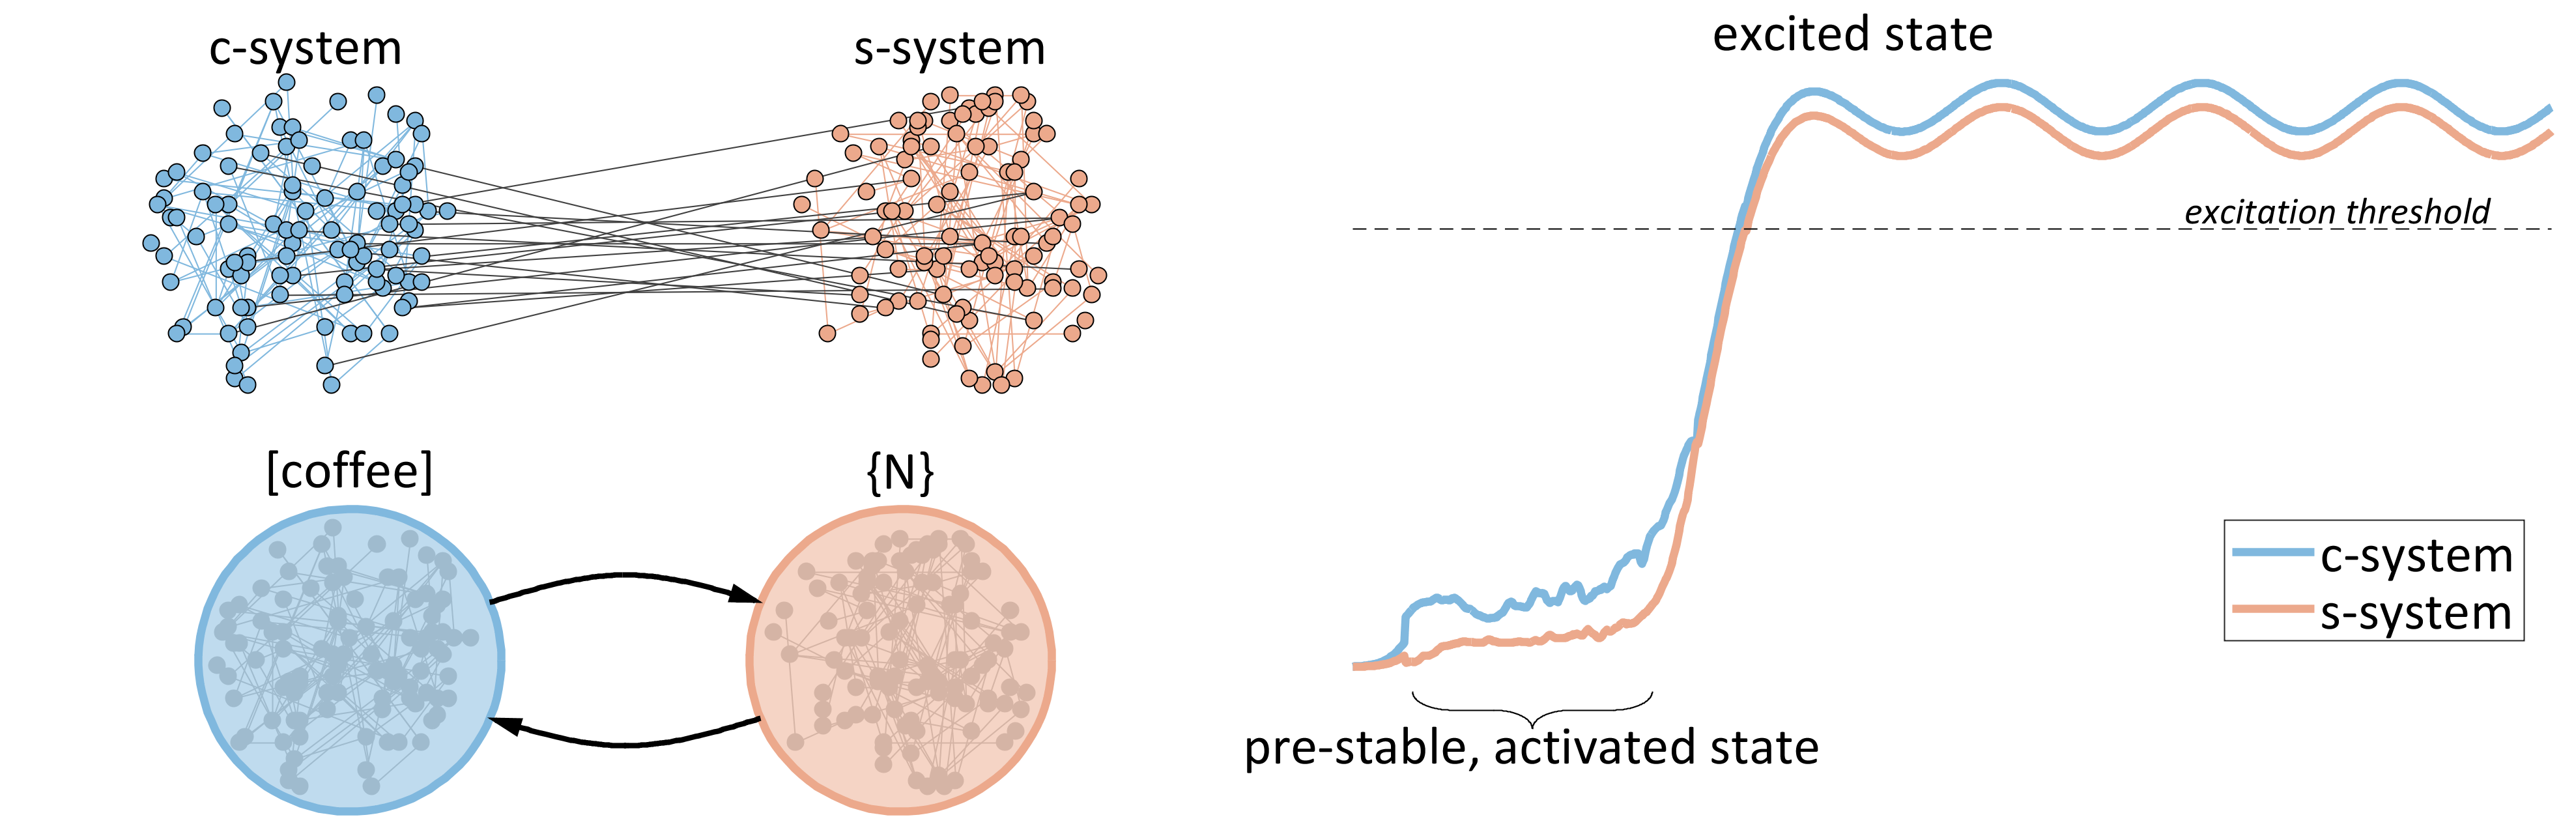
\includegraphics[width=\textwidth]{figures/Tilsen-img17.png}
\caption{\missingcaption}
\label{fig:}
\end{figure}
 

  A key diagnostic of cs-system excitation is intrapopulation and interpopulation spectral coherence, a concept which we develop in more detail later on. Moreover, the stabilization of φ entails an augmentation of \textit{e}. The excitation threshold plays an important role in a variety of analyses we develop subsequently. When a cs-system has below-threshold excitation (i.e. the system is active but not excited), the system cannot participate in a stable φ configuration with other cs-systems and hence cannot evoke an attended relational meaning experience. In general, we imagine that there are many active but unexcited cs-systems, before and during production. Thus, in the production of an utterance such as \textit{Al drinks coffee}, the excitation of [Al], [drinks], and [coffee] is merely the tip of an iceberg: a large amount of subthreshold activity occurs below the surface.

\subsection{Coupling force types and valence} 

To classify interactions between systems, we distinguish two types of coupling and two coupling valences. Relative phase coupling (φ-coupling) is an interaction that depends on relative phase φ and influences θ variables. The {\figurebelow} shows the phases of two systems on a phase circle, which is the space of possible phases. The effects of the relative phase (φ) coupling force are shown by the arrows: an attractive φ-force drives θ variables (which are also rotating counterclockwise) toward one another, resulting in a decrease in φ; a repulsive φ-force drives θ variables away from one another, resulting in an increase in φ. The coupling force is associated with a periodic sinusoidal potential function V(φ), such that  $F\left(\varphi \right)=\frac{-\mathit{dV}\left(\varphi \right)}{\mathit{d\varphi} }$ . The effect of the force on φ is analogous to a ball rolling down a hill while submerged in a viscous fluid, where the viscous force perfectly compensates for inertia: the force causes φ to change until it reaches the stable equilibrium of 0 (attractive force) or ±π (repulsive force), where it stops. Because θ is a periodic variable, it is convenient to map φ to the interval [-π,+π]. 

  
\begin{figure}
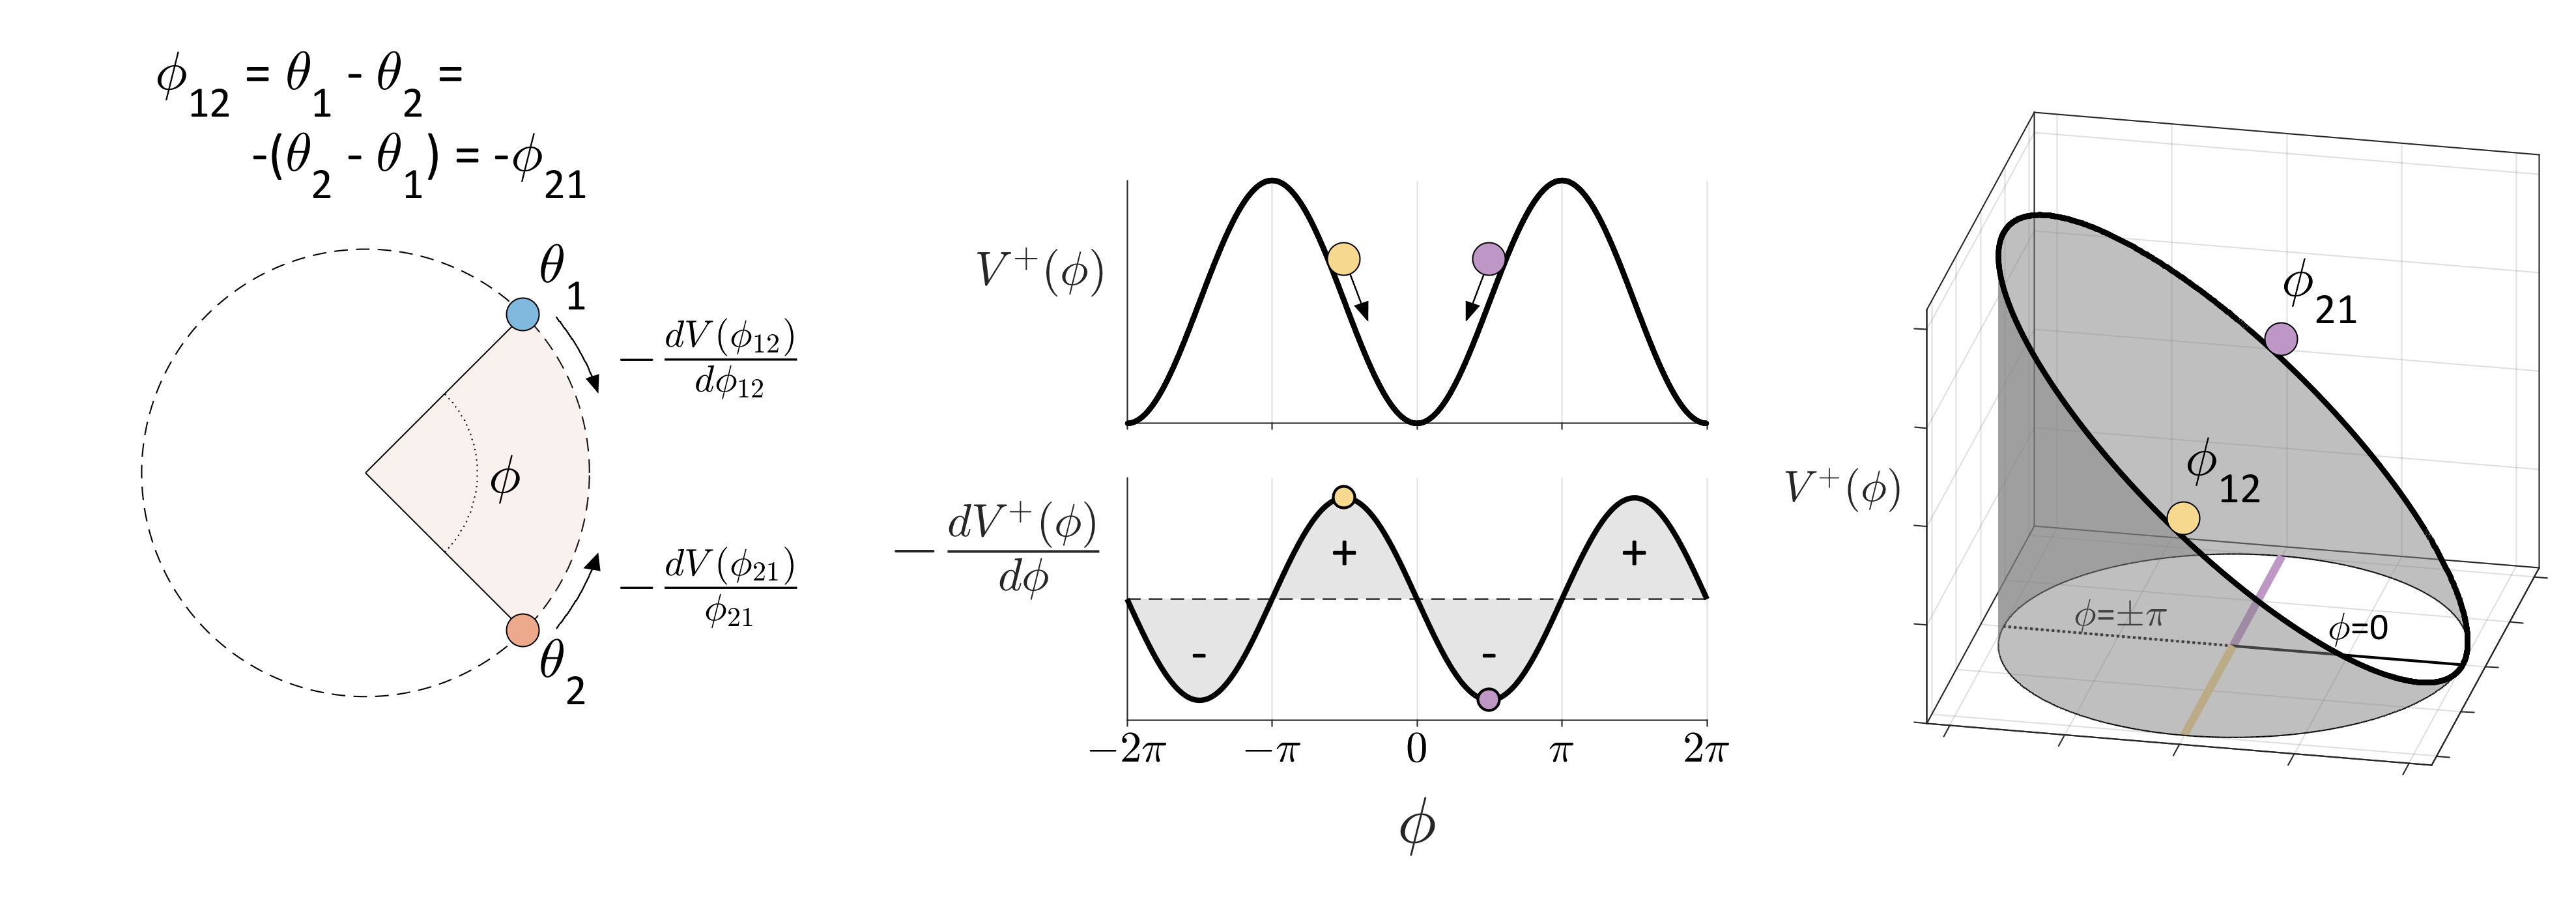
\includegraphics[width=\textwidth]{figures/Tilsen-img18.png}
\caption{\missingcaption}
\label{fig:}
\end{figure}
 

  
\begin{figure}
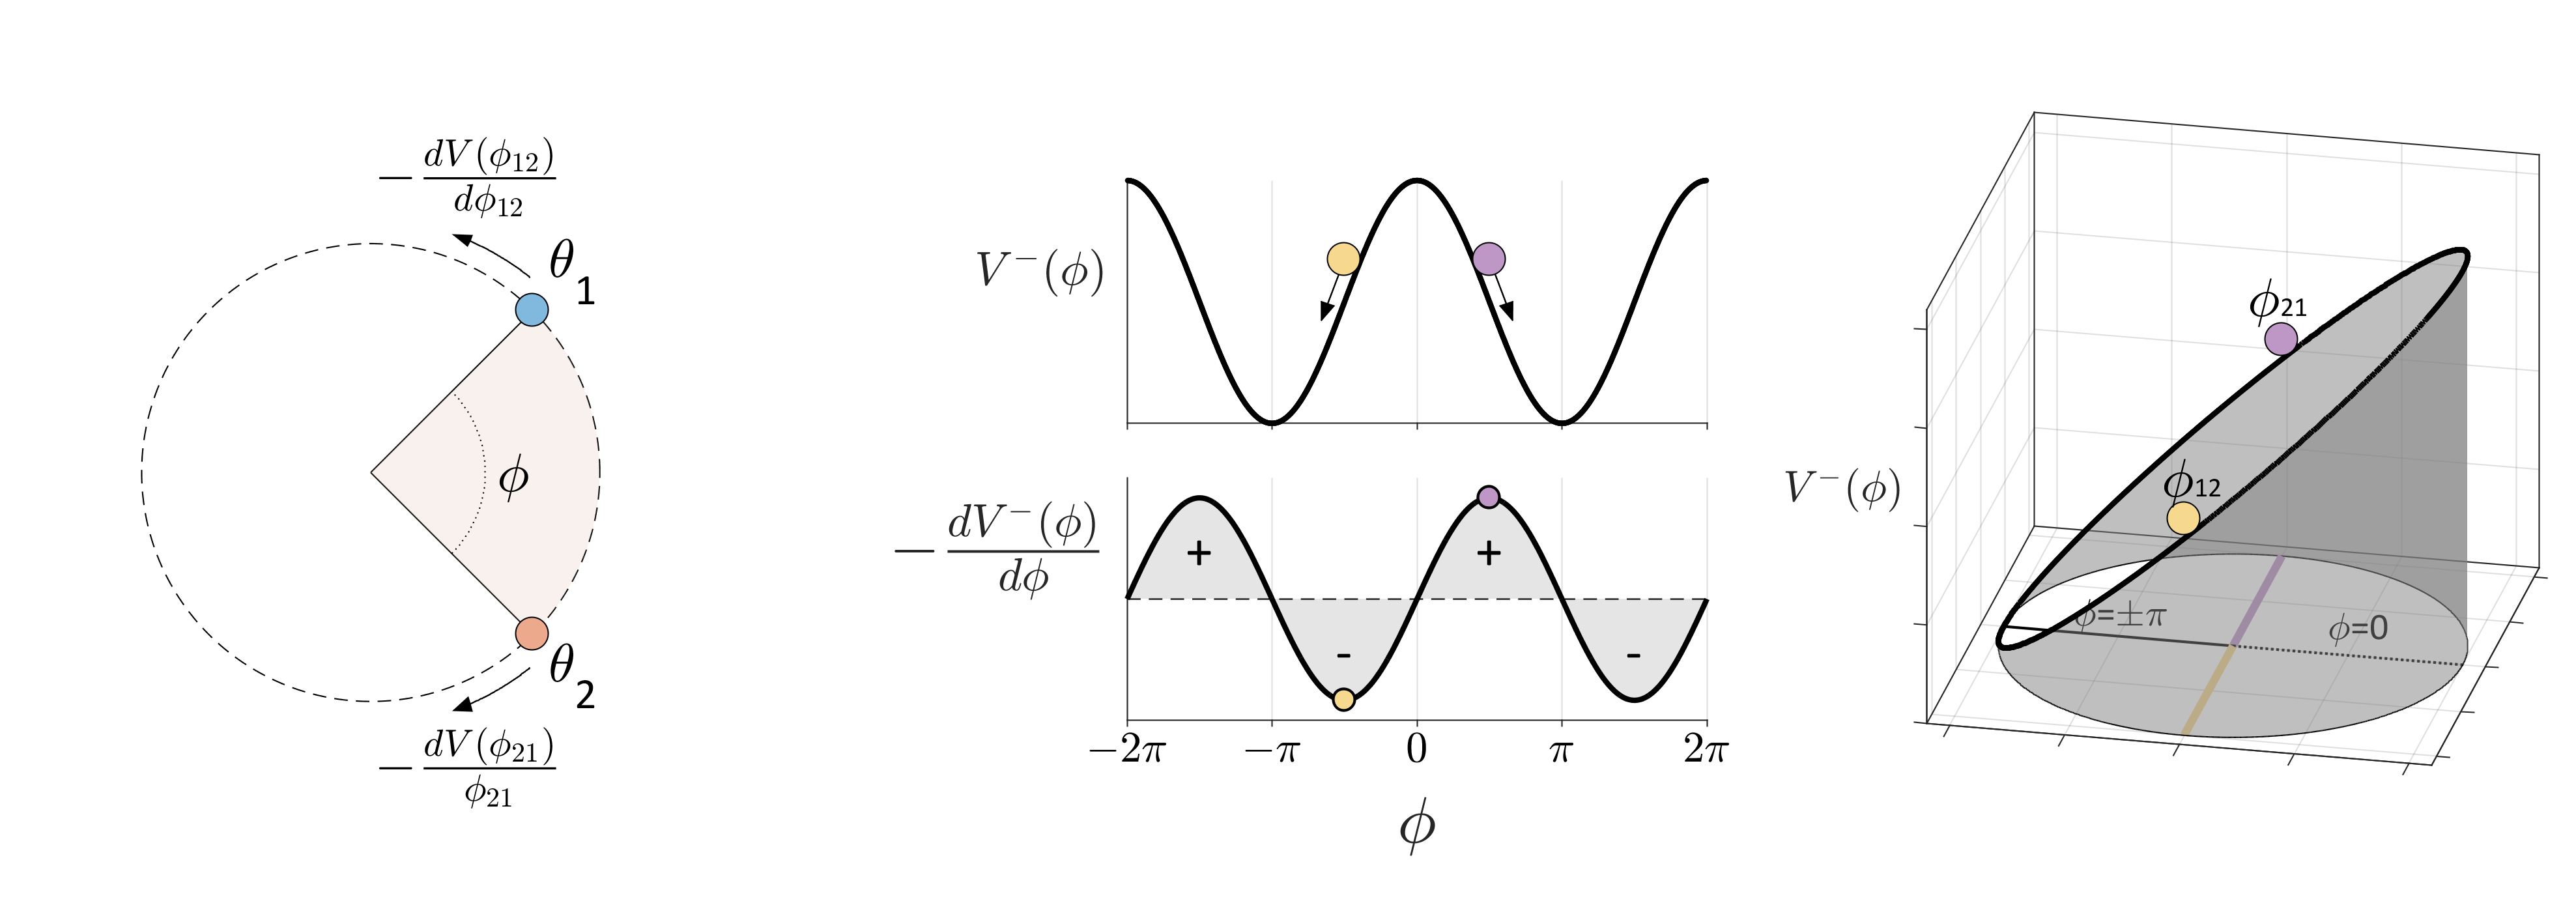
\includegraphics[width=\textwidth]{figures/Tilsen-img19.png}
\caption{\missingcaption}
\label{fig:}
\end{figure}
 

  The other type of force is excitation coupling (e-coupling). Excitation coupling is an interaction which depends on and influences \textit{e} variables. An excitatory e-coupling force results in each system increasing the \textit{e} value of the other, and an inhibitory e-coupling force results in the each system decreasing the \textit{e} value of the other. We do not specify a functional form for this force, as its role in the current framework is not well developed and is generally secondary to other mechanisms.

  Both φ-coupling and e-coupling forces can have positive [+] or negative [-] valence, as schematized below. An attractive (+φ) force causes the θ of systems to become more proximal and a repulsive (-φ) force causes θ to become more distal. An excitatory (+e) force causes \textit{e} values to increase, and an inhibitory (-e) force causes \textit{e} values to decrease: 

  
\begin{figure}
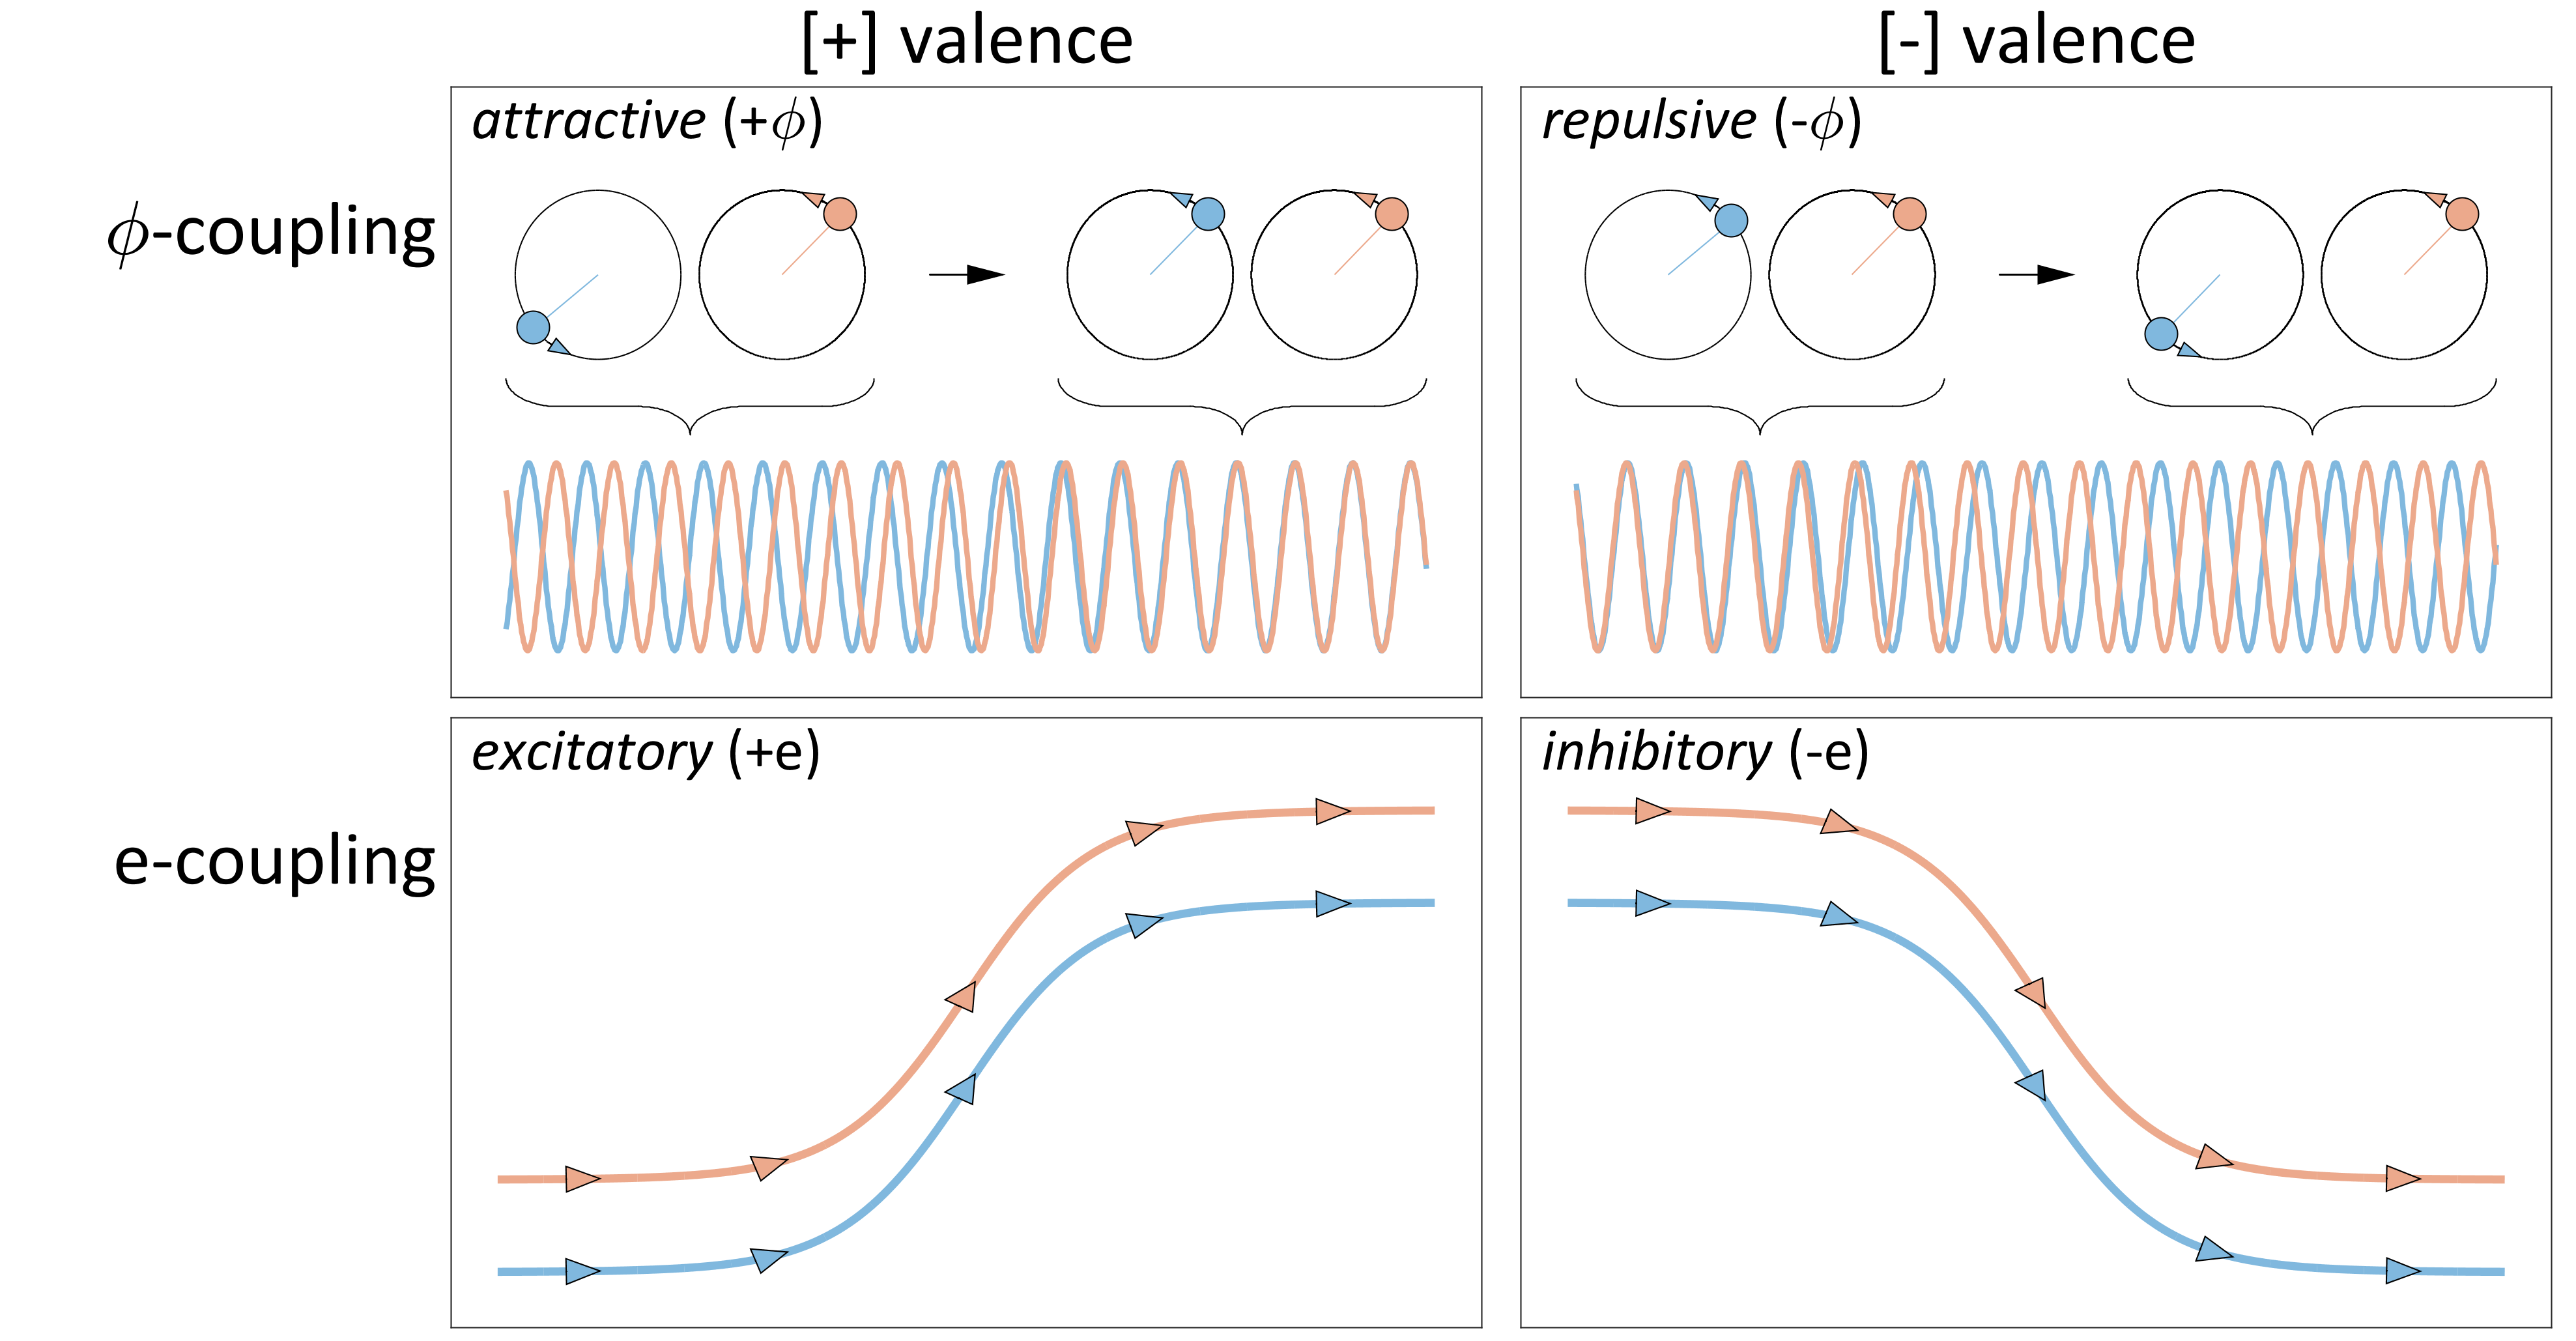
\includegraphics[width=\textwidth]{figures/Tilsen-img20.png}
\caption{\missingcaption}
\label{fig:}
\end{figure}
 

  The equations below show the roles of φ- and e-forces in influencing how θ and \textit{e} variables change in time. The total φ- and e-forces a system experiences are sums over forces from pairwise interactions with other systems, plus forces from the surroundings, \textit{S}. These forces have coupling strengths/susceptibilities φ and $\varepsilon $, respectively. The φ-force from \textit{S} is negligible, because the surroundings are too large to exhibit a collective oscillation. However, the surroundings can exert non-negligible e-forces. The term \textit{f} is an intrinsic frequency of the system (angular velocity \textit{ω} = 2π\textit{f}), representing population-internal forces which promote collective oscillation. The operator  $\widehat {{E}}\left[\overrightarrow{{\theta} },\overrightarrow{{e}}\right]$ is a placeholder for mechanisms of e-organization, and we develop these in detail later on.

\begin{equation*}
{\acute{{\theta} }}_{i}={2\mathit{\pi f}}_{i}+{F}_{\mathit{\varphi S}}\left(S,{\theta} _{i}\right)+\sum _{j}{{{\Phi} _{\mathit{ij}}F}_{\varphi} \left({\varphi} _{\mathit{ij}},{e}_{i},{e}_{j}\right)}
\end{equation*}
\begin{equation*}
{\acute{{e}}}_{i}=\text{Ê}\left[\overrightarrow{{\theta} },\overrightarrow{{e}}\right]+{F}_{\mathit{eS}}\left(S,{e}_{i}\right)+\sum _{j}{{{\varepsilon} _{\mathit{ij}}F}_{e}\left({\varphi} _{\mathit{ij}},{e}_{i},{e}_{j}\right)}
\end{equation*}

  Some properties of φ- and e-coupling can be derived from our microscale conceptualization. For one, the valences of φ- and e-forces (i.e. the signs of elements of matrices φ and $\varepsilon $) are correlated: attractive and mutually excitatory coupling tend to co-occur, and repulsive and mutually inhibitory coupling tend to co-occur. The basis for this correlation is the association of [+] valence forces with predominantly excitatory post-synaptic targets of interpopulation synapses, and conversely the association of [-] valence forces with predominantly inhibitory neurons as post-synaptic targets. These microscale patterns are illustrated below. When the excitatory neurons in population A project primarily to excitatory neurons in population B, the effect of spikes of those neurons is to attract θ\textsubscript{B} to θ\textsubscript{A} and augment \textit{e}\textsubscript{B}; when excitatory neurons in B project primarily to inhibitory neurons in B, their effect is to repel θ\textsubscript{B} from θ\textsubscript{A} and diminish \textit{e}\textsubscript{B}. 

  
\begin{figure}
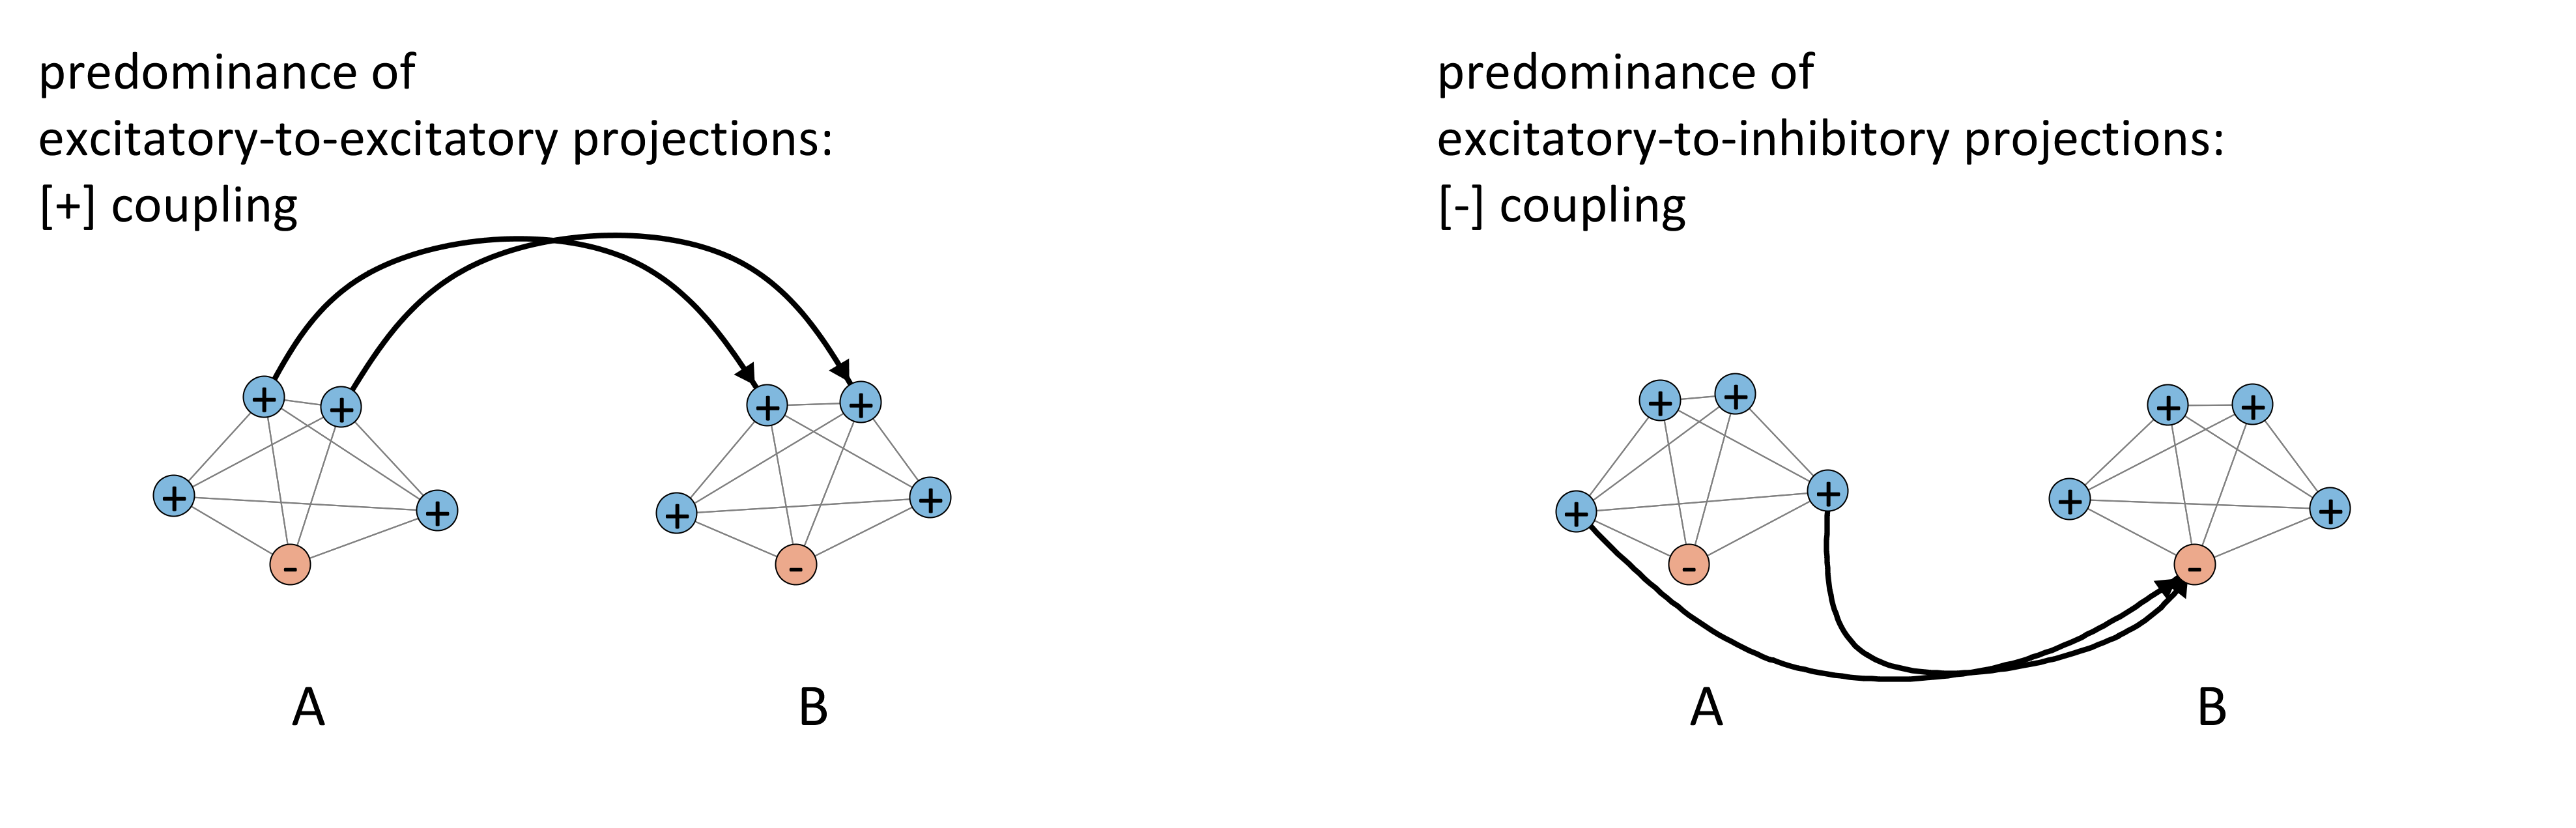
\includegraphics[width=\textwidth]{figures/Tilsen-img21.png}
\caption{\missingcaption}
\label{fig:}
\end{figure}
 

  The correlation of φ and $\varepsilon $ and valence implies that φ- and e-forces depend on both φ and \textit{e} values of systems. However, we offer no specific form for the φ-e interaction here because it would be too speculative. Nonetheless, our hypothesis that relational meaning experiences require the relevant cs-systems to be in an excited state can be viewed as a hypothesis that φ-coupling forces are modulated by \textit{e} values: the φ-forces exerted by unexcited systems are too weak to stabilize φ configurations, while systems with above-threshold \textit{e} values can exert φ-forces on one another that are sufficiently strong to induce a high degree of cs-system coherence.

  The φ- and e-coupling force matrices φ and $\varepsilon $ are also sign-symmetric. The basis for this is that Hebbian learning between bidirectionally coupled populations would be unstable on long timescales, if the valences of interactions between those populations were asymmetric. For instance, imagine a population A that is +φ coupled to population B, while B is -φ coupled to A. Spike-timing dependent learning would strengthen synapses which promote attraction of θ\textsubscript{B} to θ\textsubscript{A}, but also strengthen synapses which promote repulsion of θ\textsubscript{A} from θ\textsubscript{B}, leading to an unstable interaction in which A chases B while B runs away. Thus valence-symmetry is expected for a pair of systems. In contrast, there is no reason to expect a high degree of correlation in pairwise coupling strength for either φ- or e-coupling forces. These strengths are derived from numbers of synapses (or synaptic density, i.e. average number of synapses per neuron). To summarize, the elements of φ are correlated in sign and magnitude with those of $\varepsilon $, and within each matrix there is sign symmetry but not a high degree of correlation.

\subsection{The syntactic mechanism for organizing relational meaning}

With the conceptual tools outlined above we can construct a new understanding of the flexible emergence of relational meaning experiences. The key idea is that stable, invariant φ configurations between c-systems are created indirectly through their cs-resonances with strongly coupled s-systems. The coupling structure and phase circle representations for two example configurations are schematized below. The [Al][drinks] +φ configuration obtains because the c-system [Al] resonates with the s-system \{+N\}, the c-system [drinks] resonates with the s-system \{V\}, and the s-systems \{+N\} and \{V\} are strongly +φ coupled. Likewise, [coffee] resonates with \{-N\}, and \{V\} and \{-N\} are strongly -φ coupled.

  Although φ configurations can be decomposed into pairwise relations, multiple φ configurations which obtain simultaneously will often be shown by projecting them onto the same relative phase axis, as below. Furthermore, because the hypothesized mechanism for stabilizing φ configurations is strong φ-coupling between s-systems, the phase circle representation generally implies coupling between s-systems only; φ configurations between c-systems are an indirect consequence of strong s-system coupling. We nonetheless sometimes label c-systems on the phase circle for convenience. Because a φ configuration of c-systems entails the same configuration between the s-systems which resonate with those c-systems, we think of a φ configuration as a configuration of a cs-system. 

  
\begin{figure}
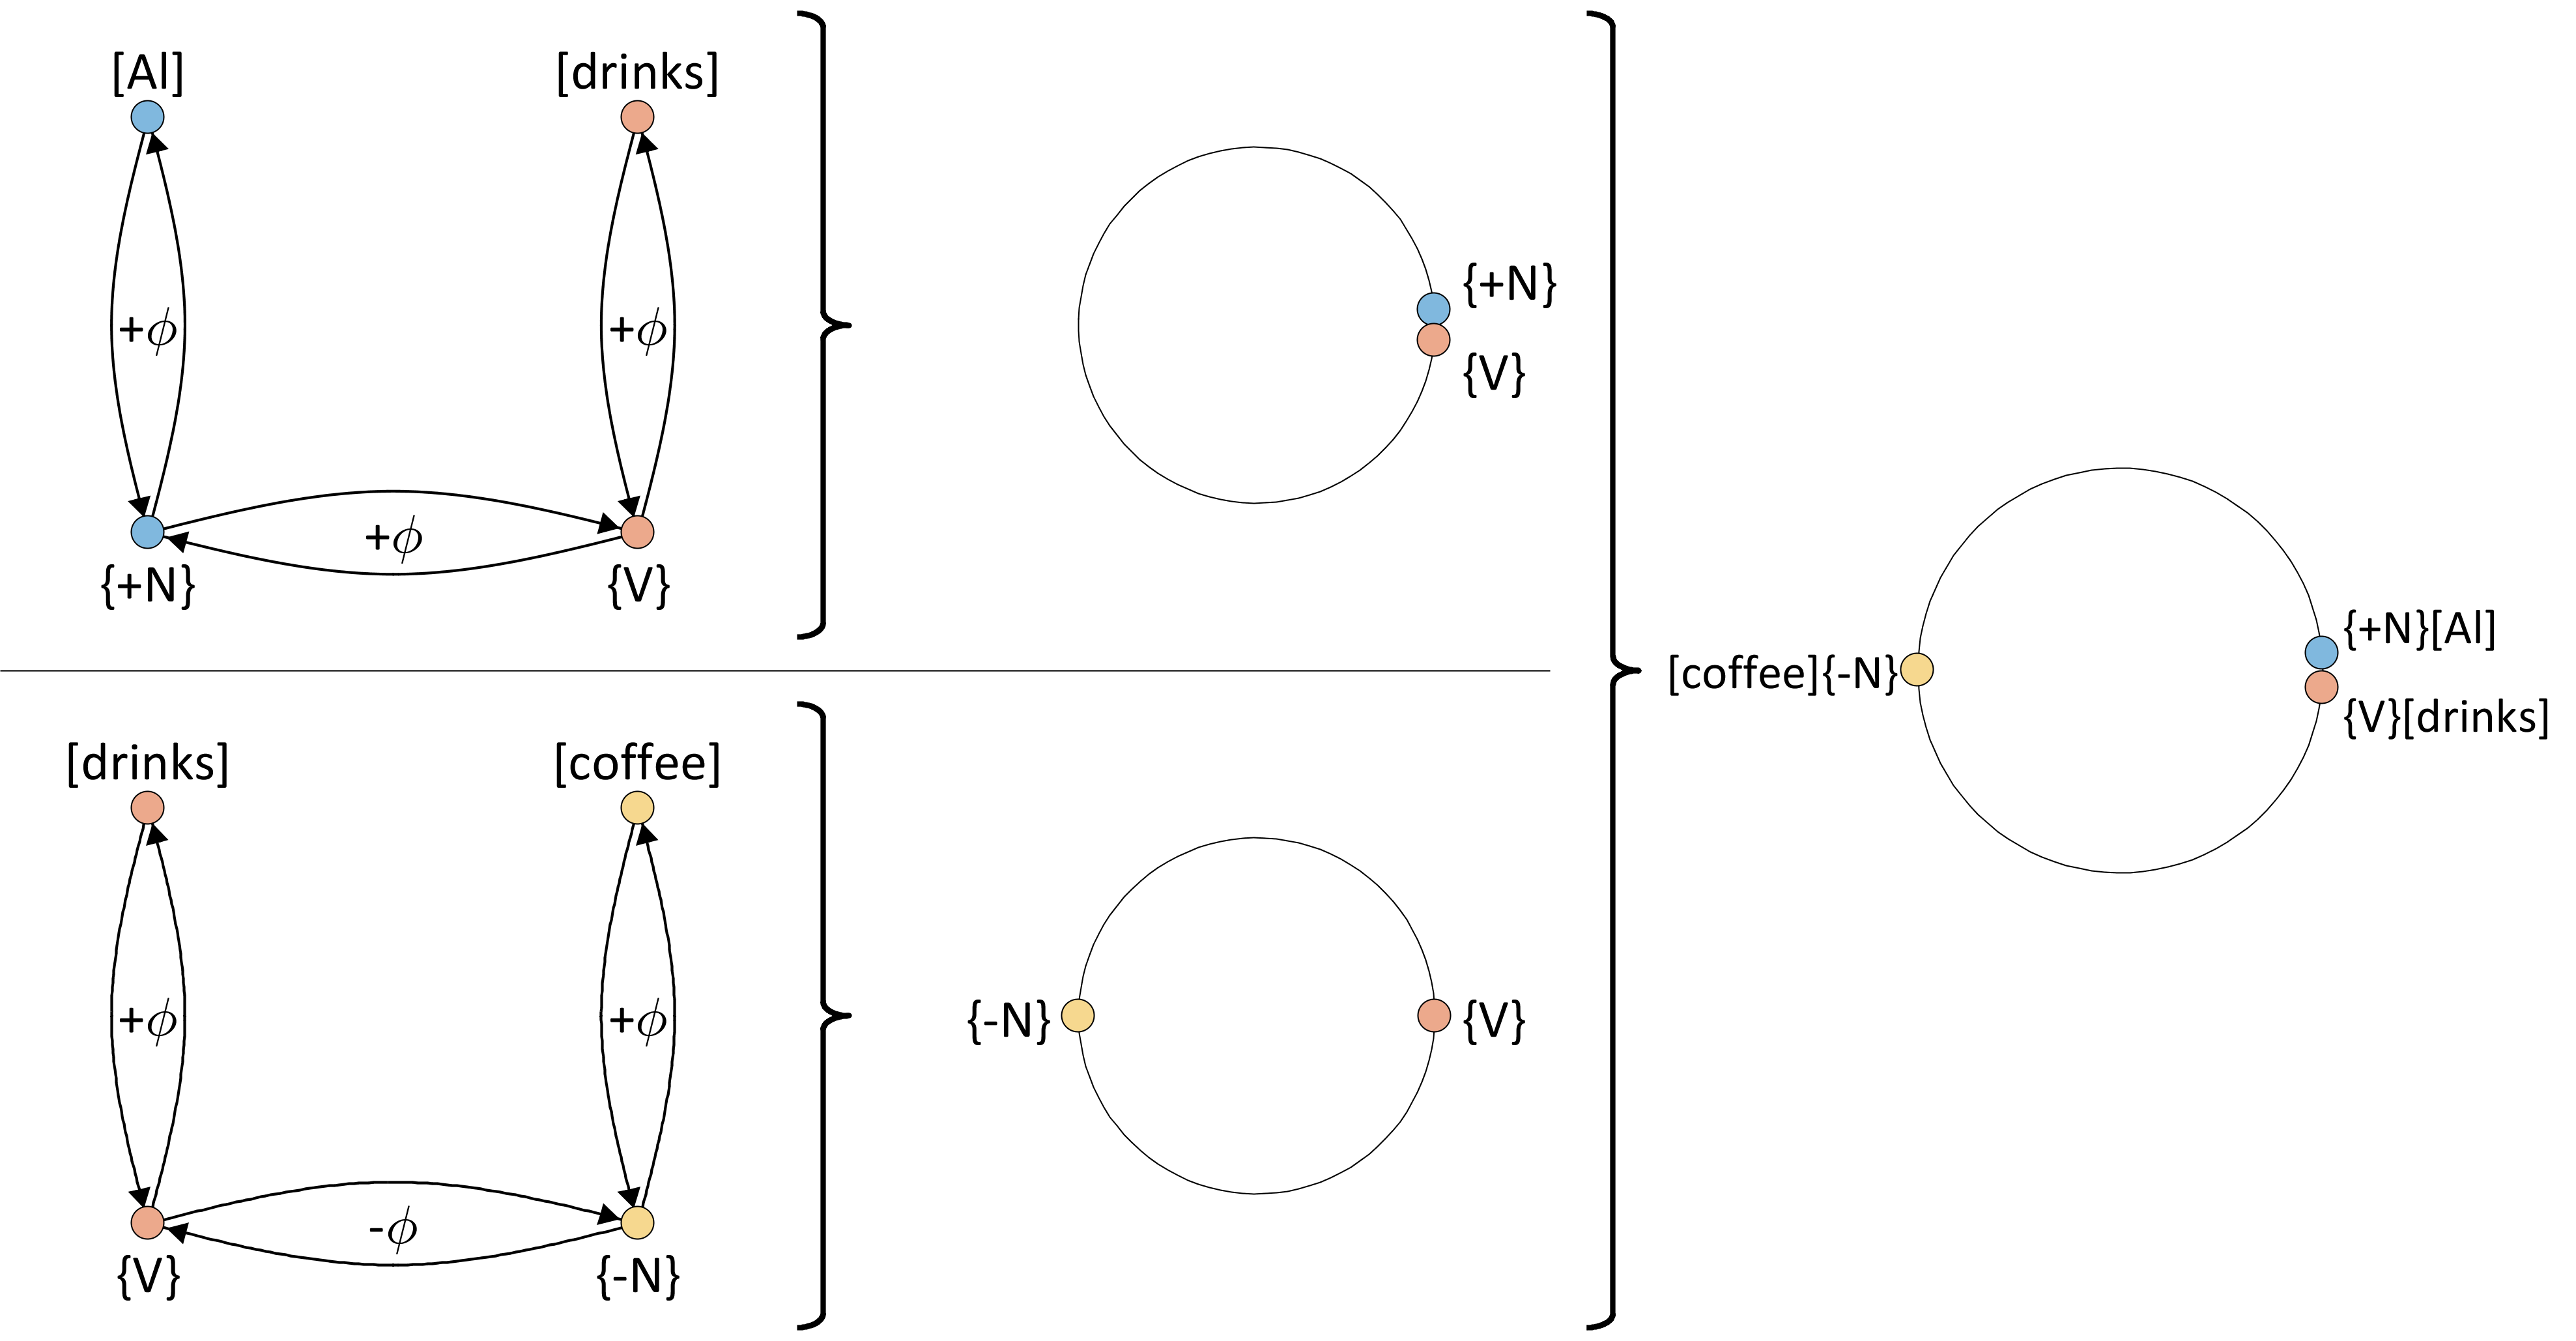
\includegraphics[width=\textwidth]{figures/Tilsen-img22.png}
\caption{\missingcaption}
\label{fig:}
\end{figure}
 

  Importantly, a φ pattern alone is not sufficient for a relational meaning experience. In addition, the pattern must be stationary in a local epoch of time. For a pattern to be stationary, there must be a stabilizing mechanism, and s-systems provide this mechanism. Recall the dynamic equation for θ. In general, the intrinsic frequencies \textit{f}\textsubscript{i} of any two systems are not the same and fluctuations in surroundings forces constantly perturb their phase velocities θ\textsubscript{i}′. In the absence of coupling forces, intrinsic frequency differences and surroundings perturbations cause φ to drift. In contrast, with the strong coupling of cs- resonances, c-system and s-system phase velocities θ\textsubscript{i}′ equalize to a compromise $\theta ′$, the value of which depends on the relative strengths of the forces and the intrinsic frequencies. This will hold as long as the coupling forces—which act to equalize phase velocity—are strong compared to the perturbing forces. Thus given sufficiently strong coupling forces, a φ configuration will remain stable.

\subsection{Interference and differentiation}

The preceding analyses distinguished between \{+N\} and \{-N\}. Why do we need to make this distinction, and how can it be understood on the microscale? The distinction between \{+N\} and \{-N\} systems (and on the microscale, \{+N\} and \{-N\} populations) is necessary because of \textit{interference}. Imagine that there is just a single, undifferentiated \{N\} population. For an utterance like \textit{Al drinks coffee}, both [Al] and [coffee] resonate with \{N\}, and [drinks] resonates with \{V\}. According to the relational meaning hypotheses presented earlier, [Al]\{N\} and [coffee]\{N\} should obtain +φ and -φ configurations with [drinks]\{V\}, respectively. These conditions are incompatible: it is not stable for \{N\} to be simultaneously +φ and -φ coupled to \{V\}.

  How does the nervous system resolve this dilemma? A crucial constraint on any solution is that populations cannot be created or added (cf. the multiplicity problem). We cannot simply posit that there is a second \{N\} population, independent of the original one. Instead, we imagine that there is one single \{N\} population, and that speakers learn to differentiate that population into \{+N\} and \{-N\} subpopulations, which are biased to +φ and -φ couple to \{V\}, respectively.

  A consequence of the differentiation mechanism is that subpopulations can \textit{interfere} with one another and become unstable. This can happen for two reasons. First, when a population is differentiated, the resulting subpopulations are smaller than the original population. The interaction forces exerted by the subpopulations on other systems become smaller, and the subpopulations themselves become more susceptible to forces from other systems and the surroundings. This can ultimately result in instability. Second, differentiated systems are not entirely independent: the corresponding subpopulations will typically overlap. The repeated differentiation of a finite population eventually results in instability, because the resulting subpopulations become smaller and have greater degrees of proportional overlap. The \{N\} > \{+N\}/\{-N\} differentiation provides two \{N\} populations which are quite stable when simultaneously excited, but when we differentiate one of these subpopulations further, stability may be threatened. The loss of stability from differentiation has important consequences which we examine in later chapters.

\section{Selection and quantal organization of excitation}

Whereas the principle of relational meaning involves organization of relative phase (φ), the principle of quantal excitation involves organization of excitation (\textit{e}). The movements associated with the production of speech arise from an organized, ordered selection of systems, determined by their relative excitation. Selection is a mechanism in which supra-threshold excitation of systems induces excitation of gestural/motor systems. Here we propose \textit{a principle of quantal excitation}: syntactic systems are organized and re-organized in a quantal relative excitation potential. This organization results in the ordered selection of motor behaviors associated with language.

\subsection{A quantal relative excitation potential}

The principle of quantal excitation is based on a conjecture that there exists a mechanism which organizes the relative excitation of s-systems into quasi-discrete, or \textit{quantal} excitation levels. We identify this mechanism with a \textit{stabilizing regime} of the excitation operator Ê in the dynamical equation for \textit{e}. The stabilizing regime of Ê is one in which \textit{e} states are mapped to themselves, and thus relative \textit{e} values remain constant. The stabilizing regime of Ê is associated with a conservative excitation potential, V(\textit{e}), as shown below for utterances \textit{Al sleeps} and \textit{Al drinks cold coffee}. 

  Observe in the examples that there are large differences in potential energy between excitation levels. The potential barriers between excitation levels entail forces which stabilize s-system \textit{e}, thereby preventing \textit{e} values from increasing to a higher level. The force that each system experiences is –dV(\textit{e})/d\textit{e}, i.e. the opposite of the derivative of the potential. The conception of force and potential energy here derives from an analogy to conservative forces, but we do not actually require a conserved quantity. Furthermore, we imagine these forces to be stationary for only for a local period of time, i.e. a single epoch of e-organization during which Ê is in the stabilizing regime. 

  
\begin{figure}
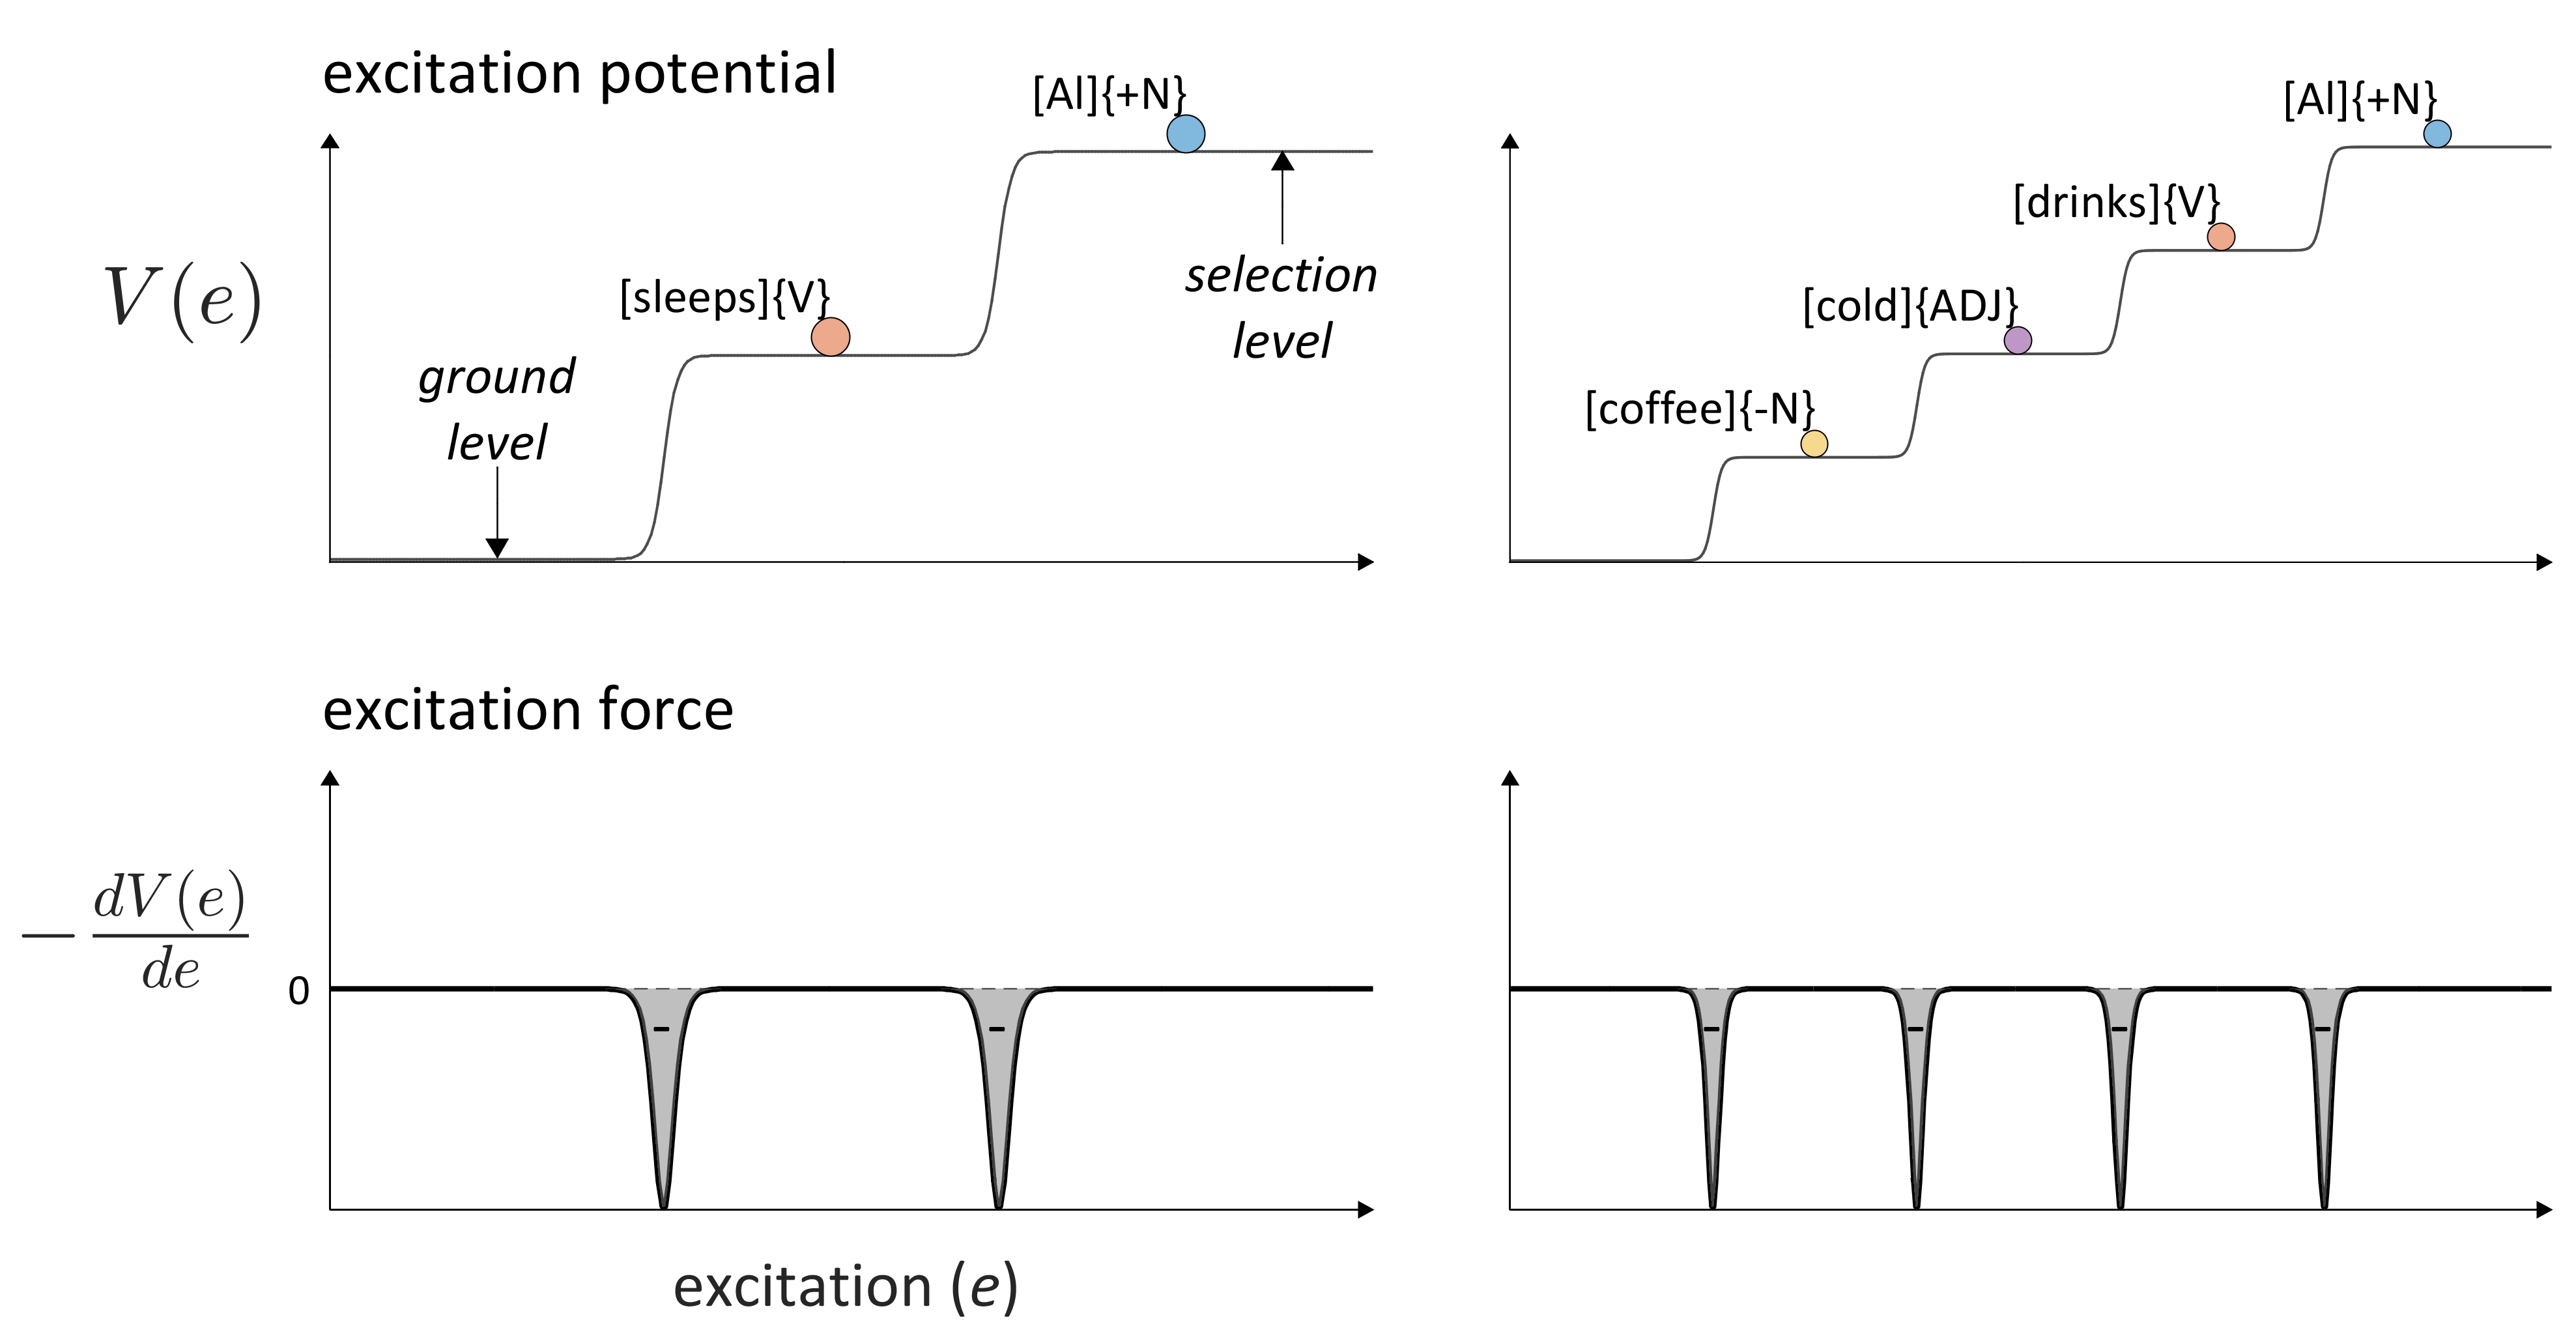
\includegraphics[width=\textwidth]{figures/Tilsen-img23.png}
\caption{\missingcaption}
\label{fig:}
\end{figure}
 

  Two levels of the potential representation have a special  interpretation. The lowest level of the potential is the \textit{ground level}, and systems on this level are by definition in an active, unexcited state. Ground state systems have at least the minimal \textit{e} value required for collective oscillation, but do not have sufficient \textit{e} to participate in a stable φ configuration. There are no “systems” below the ground level, because a system by definition is a population which exhibits collective oscillation. We distinguish \textit{ground level} systems from \textit{excited} systems, which have sufficient excitation to participate in stable φ configurations. The highest level of the potential is called the \textit{selection level}, and systems on this level have sufficient excitation to induce the selection of gestural/motor systems which are associated with a c-system. To summarize, there are three thresholds and four classes of excitation states:

\begin{table}
\begin{tabularx}{\textwidth}{llQ}
\lsptoprule
\textbf{level} & \textbf{state} & \textbf{description}\\
\midrule 
& inactive & system is undefined, no collective oscillation\\
\raggedleft ground-level & active,

non-excited & collective oscillation and minimal cs-resonance, 

\textit{e} insufficient for stable φ configuration\\
\raggedleft excitation levels & excited,

sub-selection & strong cs-resonance

\textit{e} sufficient for stable φ configuration\\
\raggedleft selection-level & selected & gates open for simulation or execution 

of associated gestural/motor systems\\
\lspbottomrule
\end{tabularx}
\caption{\missingcaption}\label{tab:key:}
\end{table}
 
 We have not addressed the question of how the quantal character of the relative excitation potential can be derived from a microscale model. Presumably, quantal e-organization manifests partly from e-coupling interactions between s-systems, and we note that the effects of the potential are reminiscent of normalization mechanisms associated with on-center/off-surround fields \citep{Grossberg1978,Grossberg1987}. However, a detailed understanding of this mechanism has not yet been developed, and the quantal potential must currently be viewed as a phenomenological approximation with primarily heuristic value. Because of this, there is no reason to commit to a particular shape of the potential, and one can imagine a number of alternatives, as below:

  
\begin{figure}
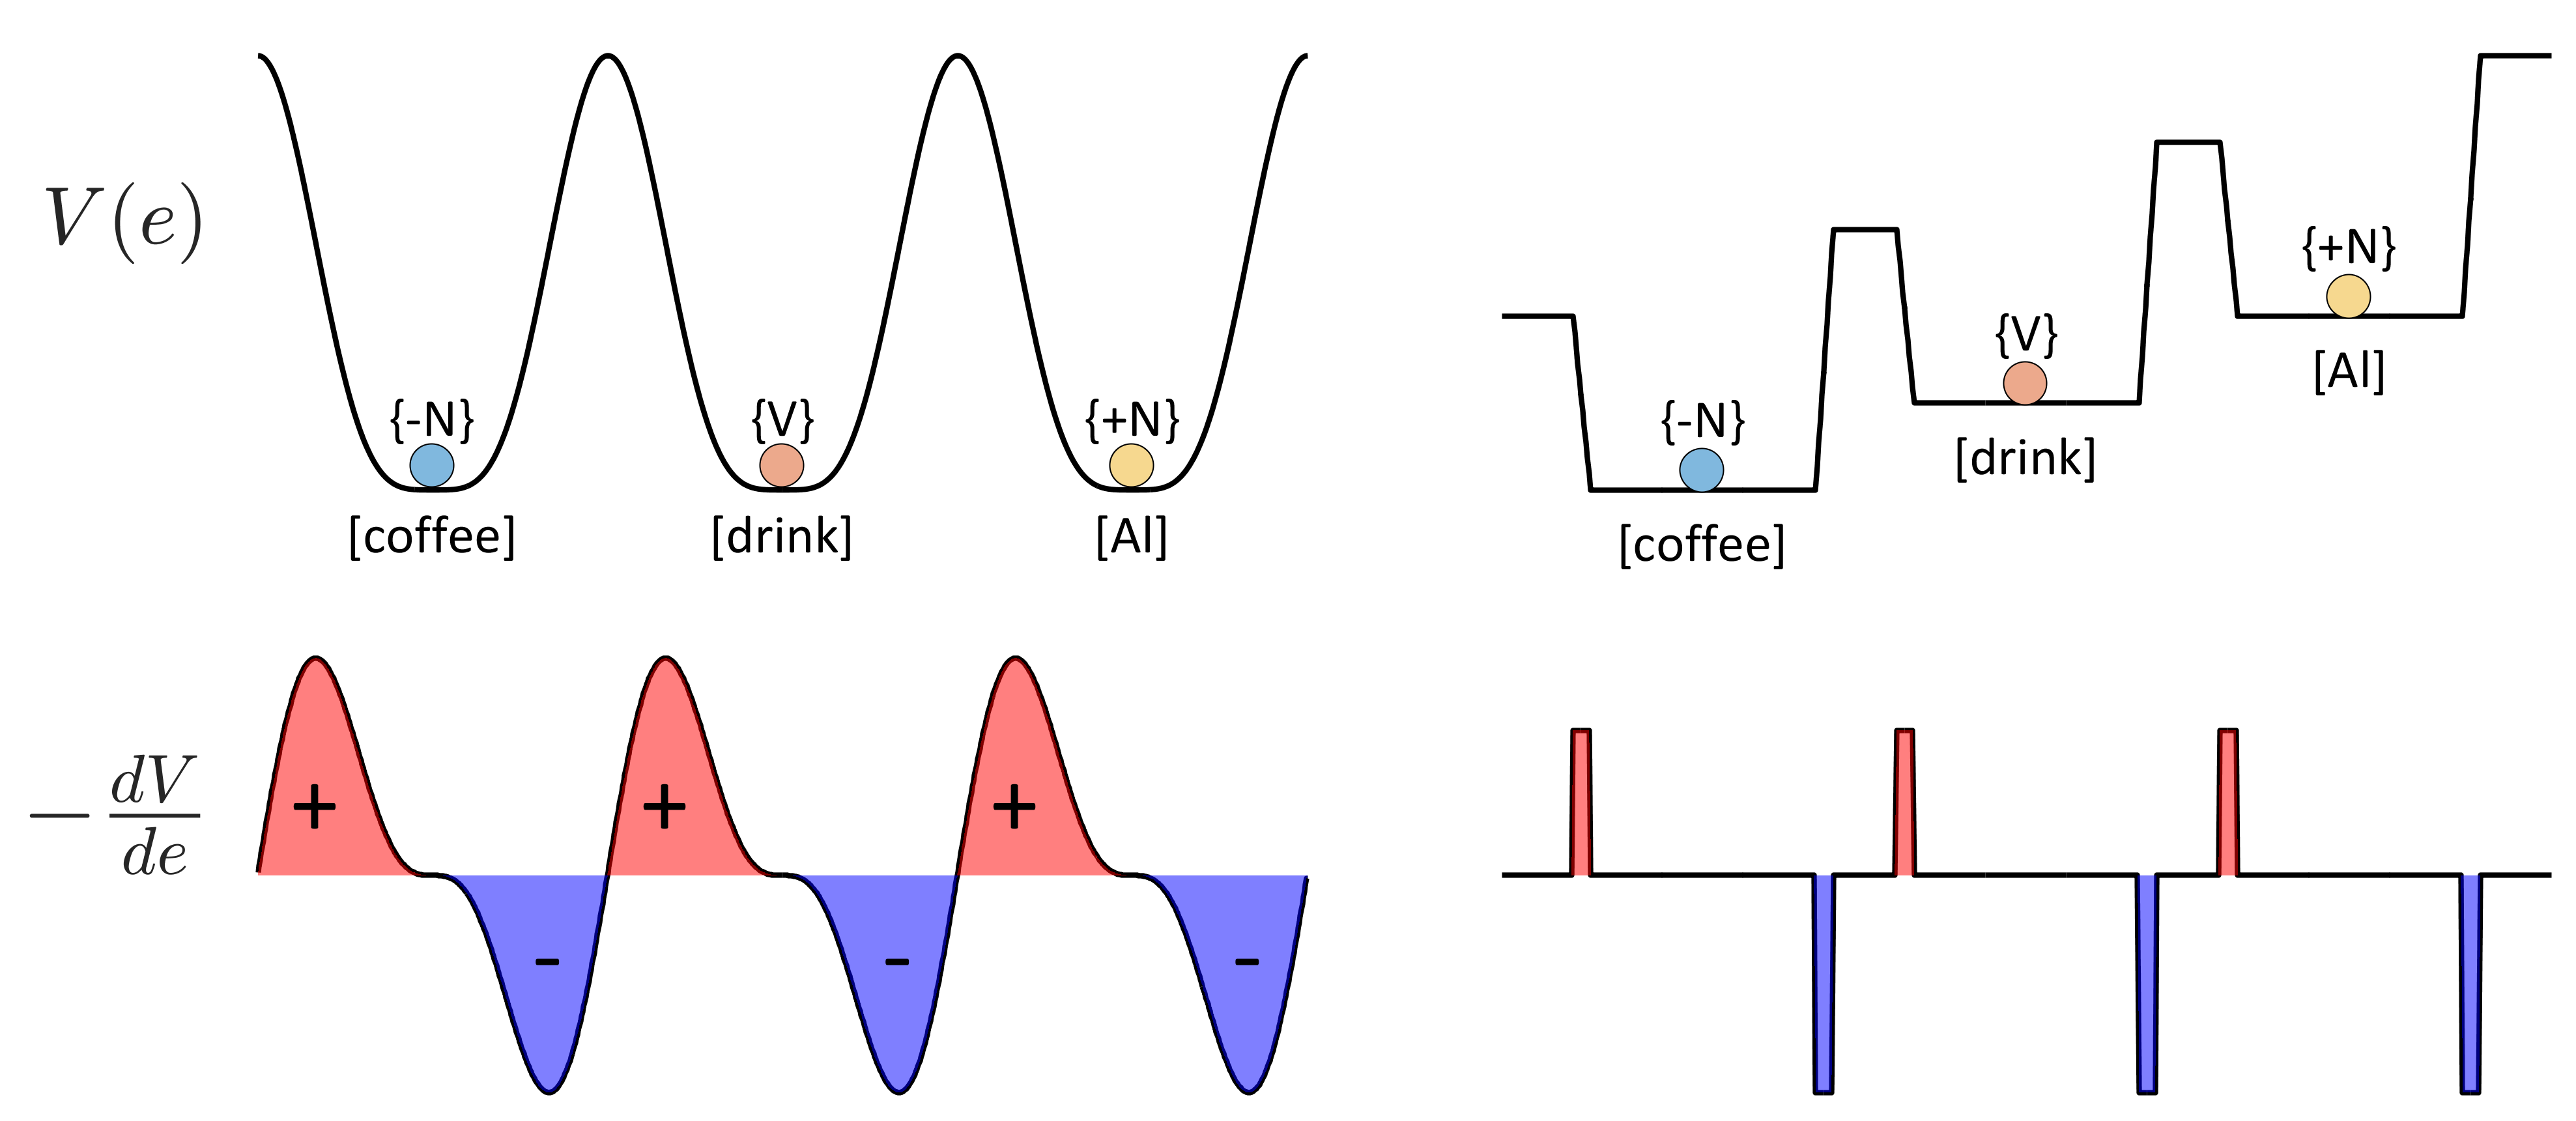
\includegraphics[width=\textwidth]{figures/Tilsen-img24.png}
\caption{\missingcaption}
\label{fig:}
\end{figure}
 

  Although the particular form of the potential function is not so important, its quantal nature is paramount, because the effect of the potential must be to stabilize a pattern of relative excitation which enforces mutual exclusivity of selection. Hence, when [Al]\{+N\} is selected, [drink]\{V\} and [coffee]\{-N\} are not selected, and so on. 

  There are several points to emphasize regarding the e-potential representations. First, as explained above, these representations are schematic and imply discretized patterns of relative excitation; they do not imply specific values or specific relative magnitudes. Second, e-potentials govern the \textit{e} values of s-systems, not c-systems. In cs-resonances, c-system \textit{e} values are correlated with s-system \textit{e} values, but the correlation is not exact. We nonetheless often label c-systems in e-potentials, for convenience, and often refer to cs-systems in this context. 

  Third, intermediate levels of an e-potential \textit{never exist independently of the systems which occupy them}. The potential is conceptualized as an emergent phenomenon associated with interactions between s-systems, and as such it is not sensible to imagine an “unoccupied level”. (The ground and selection levels are exceptions, for reasons we discuss later.) The potential levels are \textit{not} locations in space, and the systems are \textit{not} objects which occupy locations. Instead, the quantal potential is understood as a pattern of organization that is created by a combination of local interactions between s-systems and a general purpose ordering mechanism which operates on an \textit{e} value code. Rather than saying that systems \textit{occupy} levels, it is more precise to say that interactions between s-systems bring about the conditions for the stabilization of their relative excitation.

\subsection{Canonical reorganization}

While the stabilizing regime of Ê enforces an approximate temporal invariance on \textit{e}, a reorganization regime of Ê causes intermittent, abrupt changes in \textit{e}. These changes map \textit{e} configurations to \textit{e} configurations in predictable ways. Reorganization mappings cause changes in \textit{e} configuration which are discontinuities on the φ-timescale. We refer to the stable periods of time between these discontinuities as e-epochs. We are interested here in the various forms that reorganization mappings can take, and in what aspects of the system state they might depend on. In general, reorganization operations could depend on all θ and \textit{e} variables of all active and excited systems—i.e. the full system state. However, we can infer that some information is typically not relevant to the mapping. 

  The default mechanism for ordering the selection of systems is the canonical reorganization mapping, Ê\textsuperscript{cr}. θ/φ information is irrelevant for canonical reorganization. The operation  can be understood as follows, using the utterance \textit{Al drinks coffee} as an example. First, assume the initial condition in epoch (e1), an \textit{e} configuration which is stabilized by stabilization regime Ê. In epoch (e1), [Al]\{N\} has selection-level excitation, and this drives the excitation of motoric/gestural systems associated with [Al]. Feedback resulting directly or indirectly from motoric/gestural excitation eventually causes a transition to the canonical reorganization regime. The canonical re-organization mapping Ê\textsuperscript{cr} causes an abrupt change from epoch (e1) to epoch (e2), in which the selection-level system is \textit{demoted} to the lowest excited state, and all other excited systems are promoted one level. Ê\textsuperscript{cr} applies to transitions from (e2) to (e3) and from (e3) to (e4) as well. Note that Ê\textsuperscript{cr} produces a cycle when iterated: e\textsubscript{1}, e\textsubscript{2}, … e\textsubscript{n}, e\textsubscript{1}… 

  
\begin{figure}
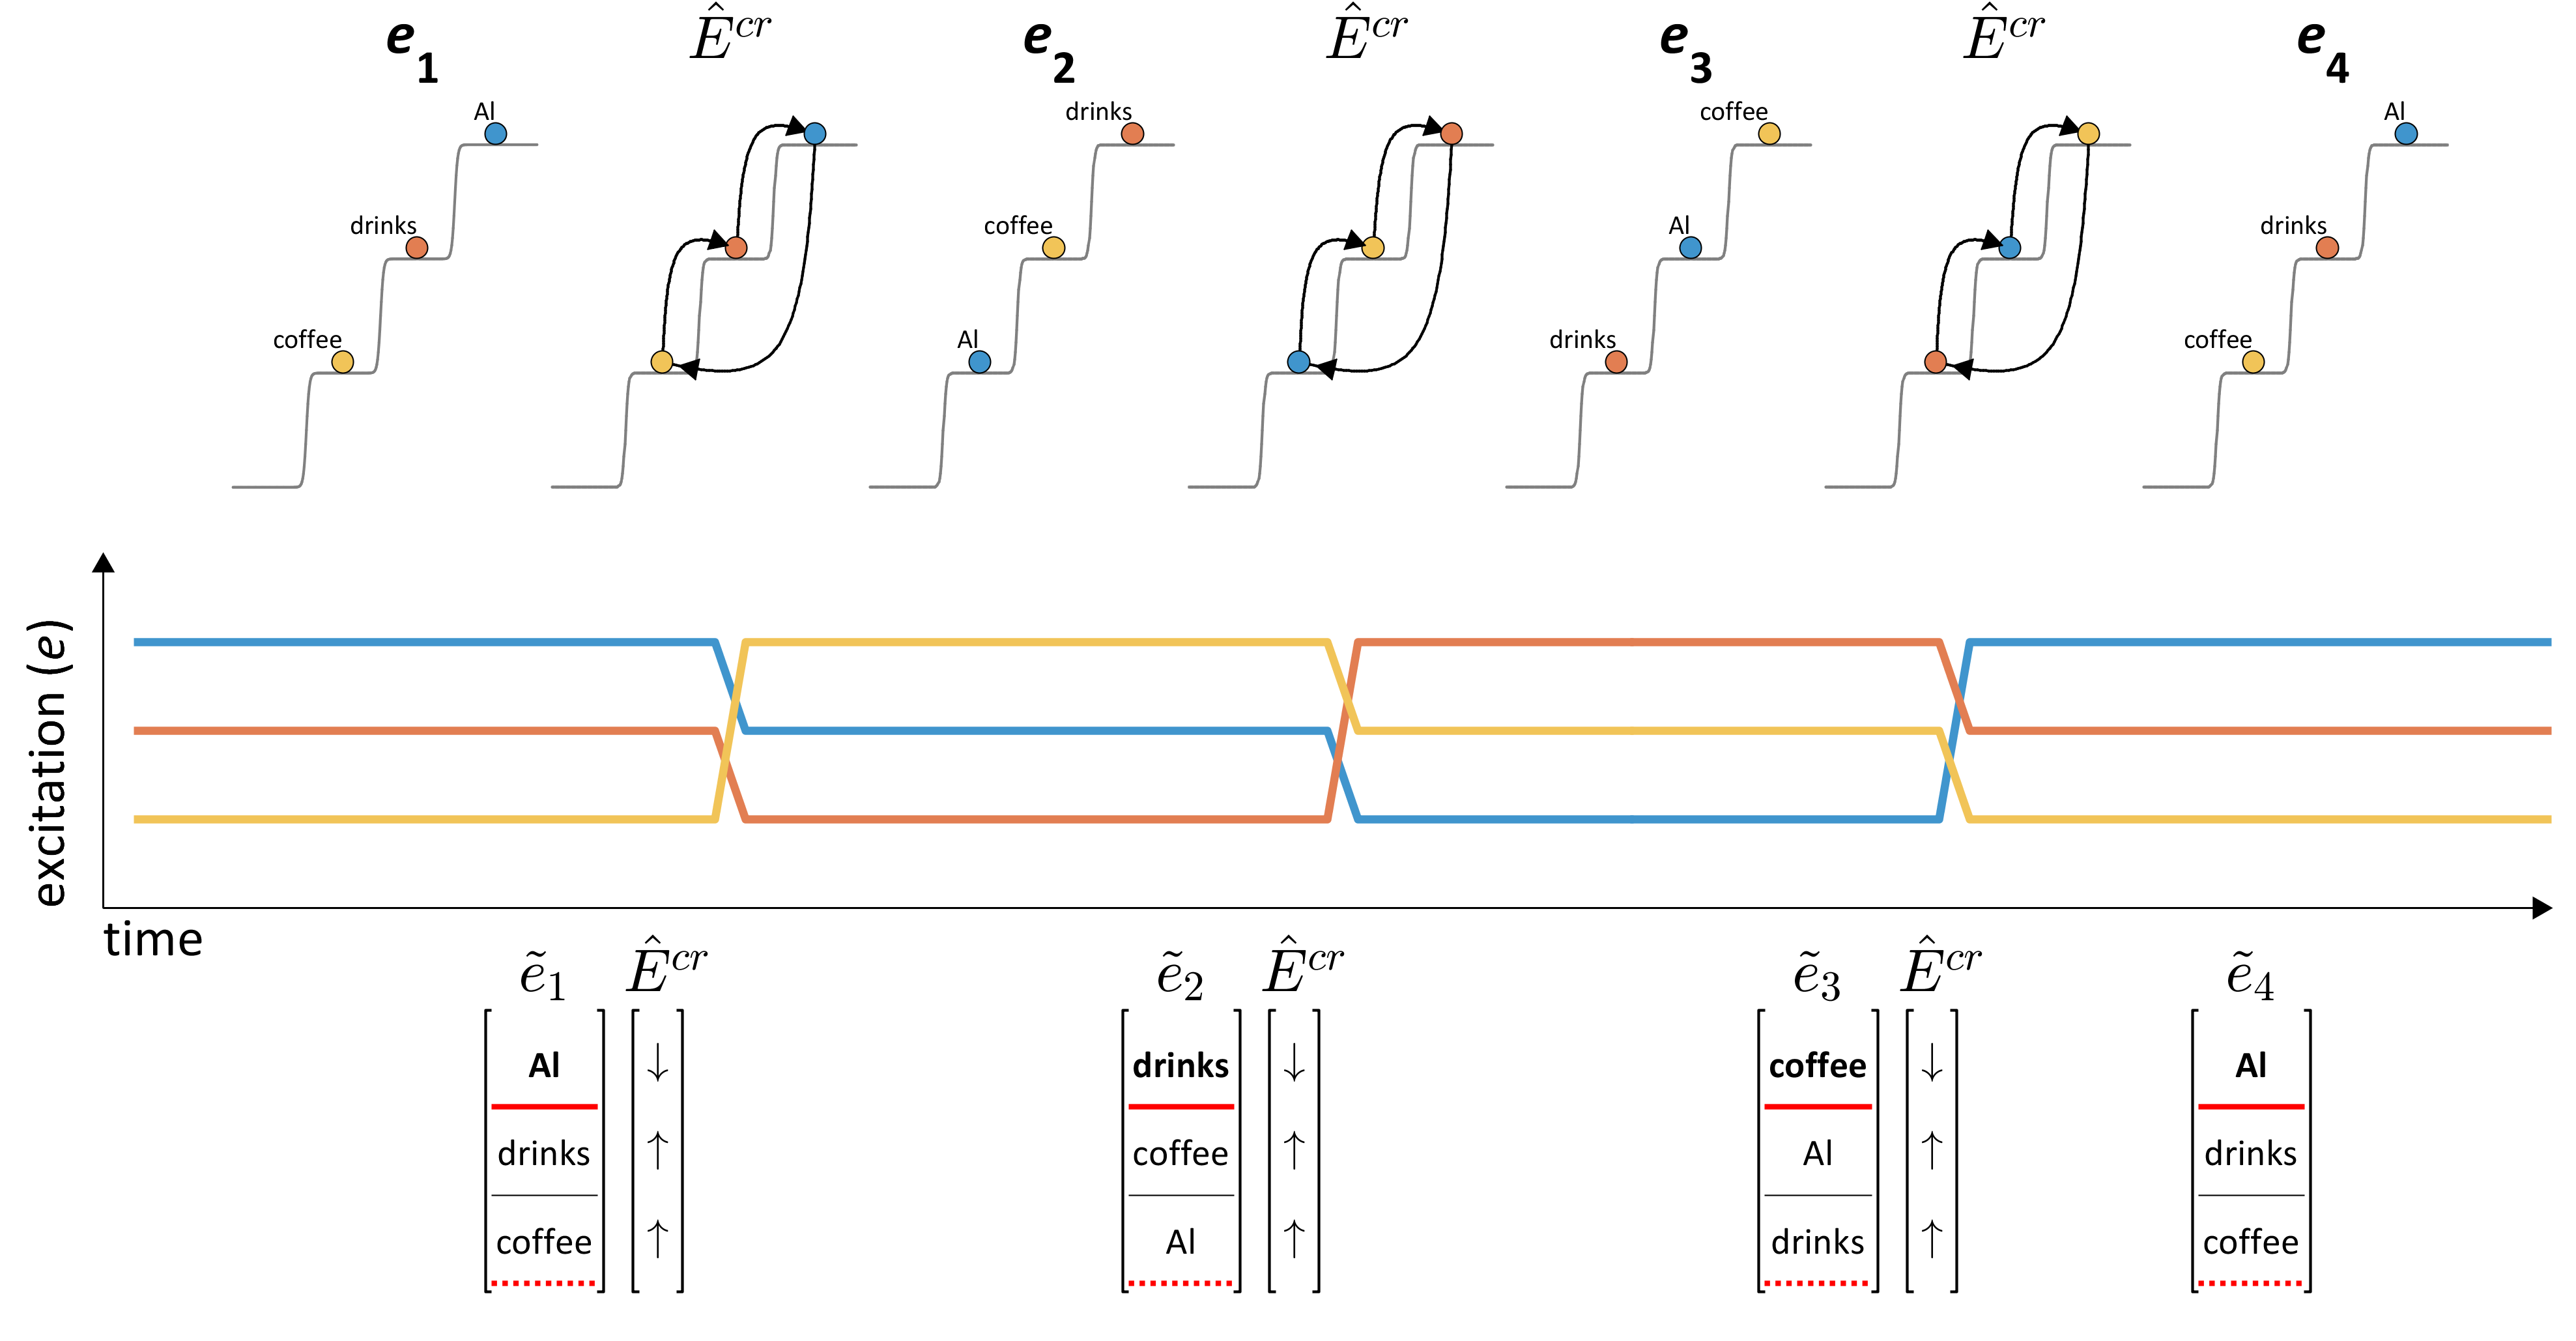
\includegraphics[width=\textwidth]{figures/Tilsen-img25.png}
\caption{\missingcaption}
\label{fig:}
\end{figure}
 

  Above we show a more compact representational formalism in which e-organization state vectors,  $\widetilde{{e}}$, are operated upon element-wise by reorganization vectors. In an e-organization state vector, systems are assigned to vector dimensions in order of their relative excitation. The figure above shows e-organization state vectors from a series of epochs. Each  $\widetilde{{e}}$ is operated upon by the canonical reorganization operator Ê\textsuperscript{cr}. The arrows in each element of Ê\textsuperscript{cr} indicate which basic operation (promotion or demotion) applies to the corresponding element of  $\widetilde{{e}}$. In this context, canonical reorganization can be understood as demotion of the most highly excited system to the lowest above-ground level, and promotion of all other systems by one level. For convenience, the excitation and selection thresholds are shown by dashed and solid red lines, respectively.

  There are a couple alternative formal approaches to representing reorganization mappings. One is to define a relative quantal excitation state vector  $\overrightarrow{{e}}$, where each dimension corresponds to a different excited cs-system. The value in a dimension is an integer from 1 to \textit{n}, where \textit{n} is the number of s-systems which occupy distinct e-levels, and the value corresponds to excitation rank order of the corresponding system. The canonical reorganization mapping in this scheme is shown below.

\begin{equation*}
{\text{Ê}}^{\mathit{cr}}\left(\overrightarrow{{e}}\right):e\rightarrow \left[e\mathit{mod}n\right]+1
\end{equation*}

  Another formalization uses a cyclic permutation matrix. In this case we define the e-state as a binary matrix Ë where each column corresponds to a level of the e-potential and each row to a system (so, a value of 1 in row \textit{n}, column \textit{m}, entails that system \textit{n} occupies excitation level \textit{m}). Repeated action of the permutation matrix Ê on Ë results in a return to the initial pattern. 

% \begin{equation*}
% \text{Ê}^{\mathit{cr}}=
% \left[
%   \begin{matrix}
%   0 & 0 & 1\\
%   1 & 0 & 0\\
%   0 & 1 & 0
%   \end{matrix}
% \right],
% {\text{Ë}}_{1}=
% \left[
%   \begin{matrix}
%   1 & 0 & 0\\
%   0 & 1 & 0\\
%   0 & 0 & 1
%   \end{matrix}
% \right]
% \end{equation*}
\todo{commented out matrix}


  The e-state vector and matrix representations are somewhat less general than the e-organization representation, for reasons that will become clear later. In contrast, the e-organization representation has greater flexibility and we make extensive use of it. The canonical reorganization is a useful construct because many of the phenomena we are interested in can be analyzed in relation to the canonical mapping.

  Although we do not attempt to model the internal dynamics of the reorganization process, we imagine promotion and demotion as brief periods of relatively strong excitatory and inhibitory forces. The picture we have in mind is below. In the stable epochs (e1) and (e2), the augmentation forces on [drinks]\{V\} and [coffee]\{N\} are not sufficient to promote these systems. But feedback regarding the selection of [Al]\{N\} induces a transition to the reorganization regime, in which there is a strong suppressive force on [Al]\{N\}, along with strong forces which augment the excitation of other systems. This may occur in combination with a reduction of the sizes of barriers in the potential. 

  
\begin{figure}
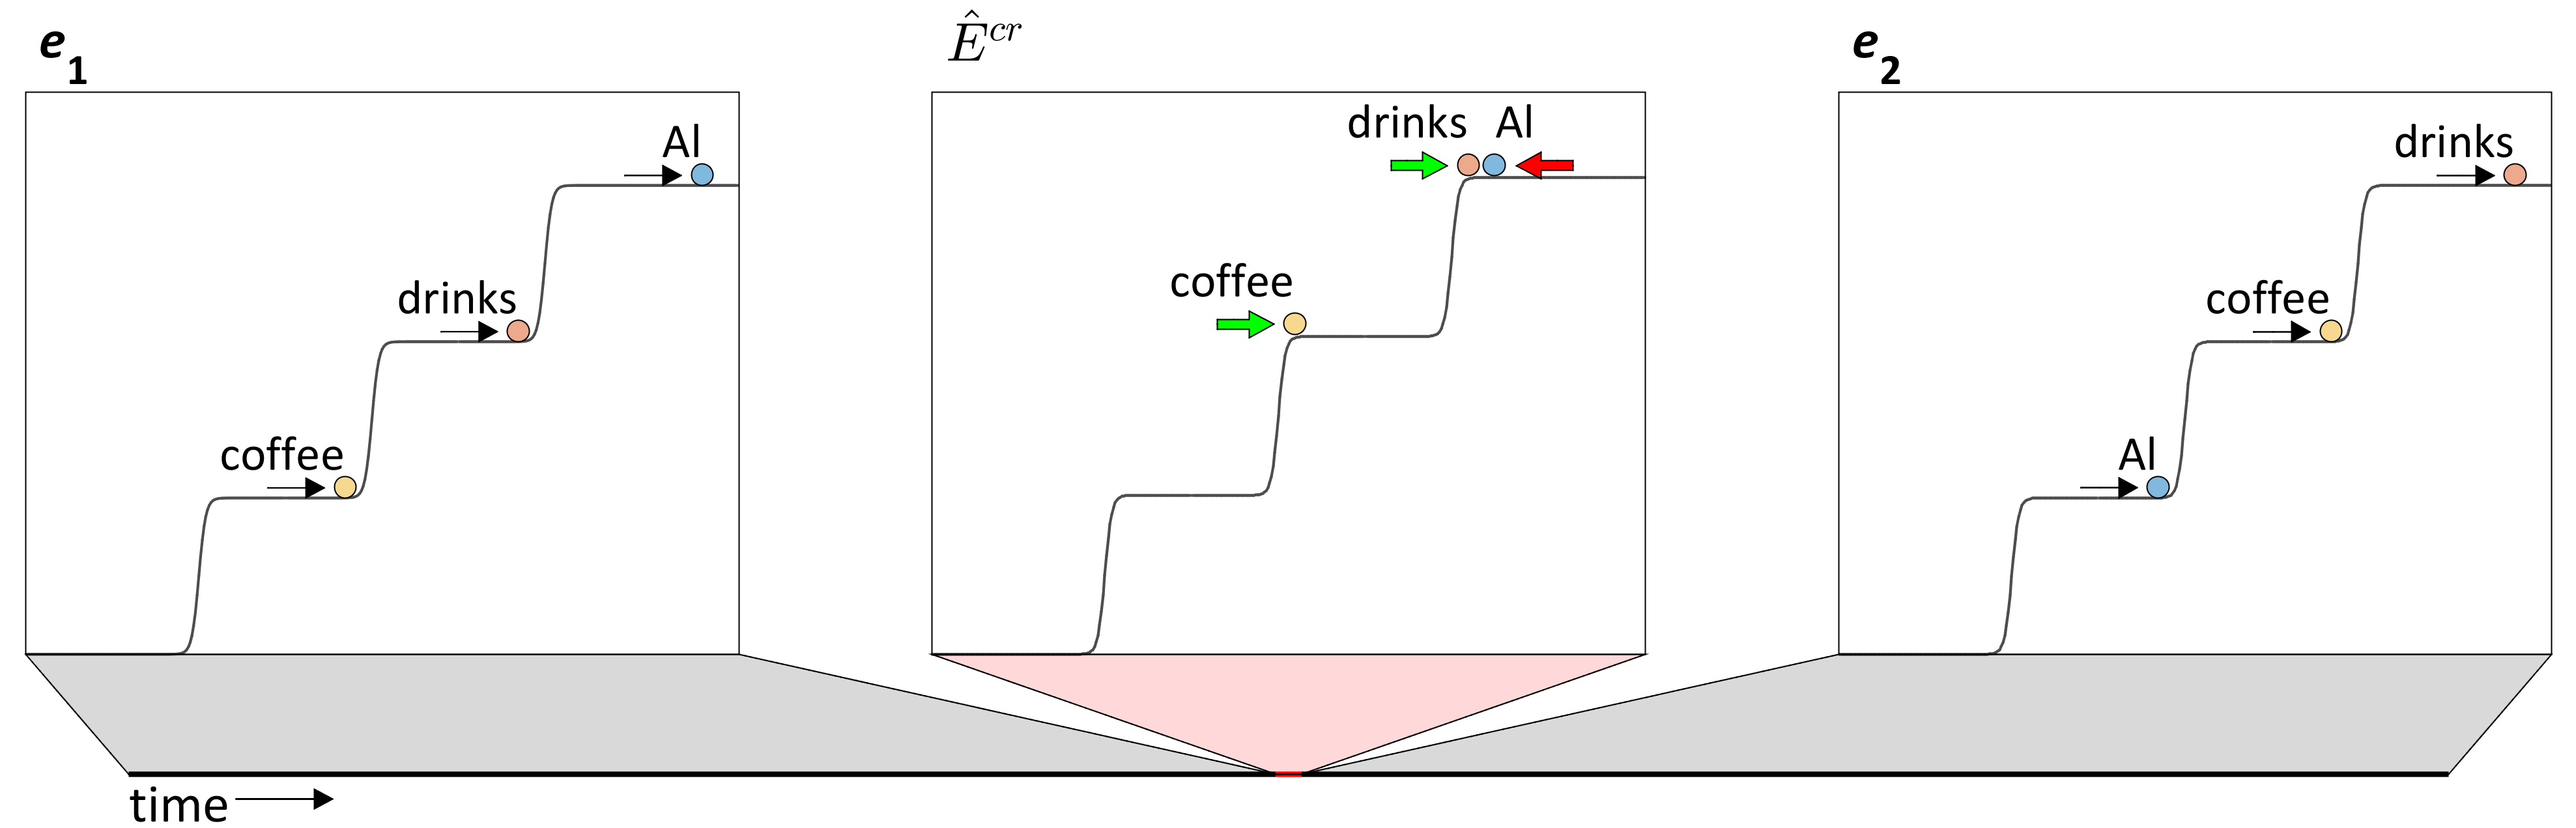
\includegraphics[width=\textwidth]{figures/Tilsen-img26.png}
\caption{\missingcaption}
\label{fig:}
\end{figure}
 

  The overall effect of the reorganization is that the \textit{e} value of the selected system, [Al]\{+N\}, decreases and the \textit{e} values of other excited systems, [drinks]\{V\} and [coffee]\{-N\}, increase. We assume that Ê returns to the stabilization regime when a new system surpasses a selection threshold, i.e. when [drinks]\{V\} is selected. It is important to emphasize that because systems are not objects, there is no sense in which there is a collision between objects. We never worry about lines crossing or objects occupying the same space in o/el representations.

\subsection{The combined picture: two conceptions of time}

The o/el framework provides two conceptual models of the temporality of speech, one which is suited for reasoning about relational meaning experiences, the other for action ordering. As shown below, a production trajectory begins with the activation of cs-systems. A stable φ configuration of excited systems then emerges in conjunction with an initial e configuration, as a result of an initial organization operator, Ê\textsuperscript{io}. (We examine mechanisms of initial organization in a subsequent chapter.) The \textit{e} configuration is then iteratively reorganized, while the φ configuration remains constant. Consequently, we see that φ-variables have a fixed point attractor throughout the trajectory (θ variables have a periodic attractor), while e-variables exhibit intermittent discontinuous changes. The steady state periods between reorganizations are e-epochs. The conceptual models of time we have constructed help distinguish between the φ-epoch timescale on which φ configurations are stable (i.e. a relational meaning experience is invariant) and the e-epoch timescale on which e configurations are stable.

  
\begin{figure}
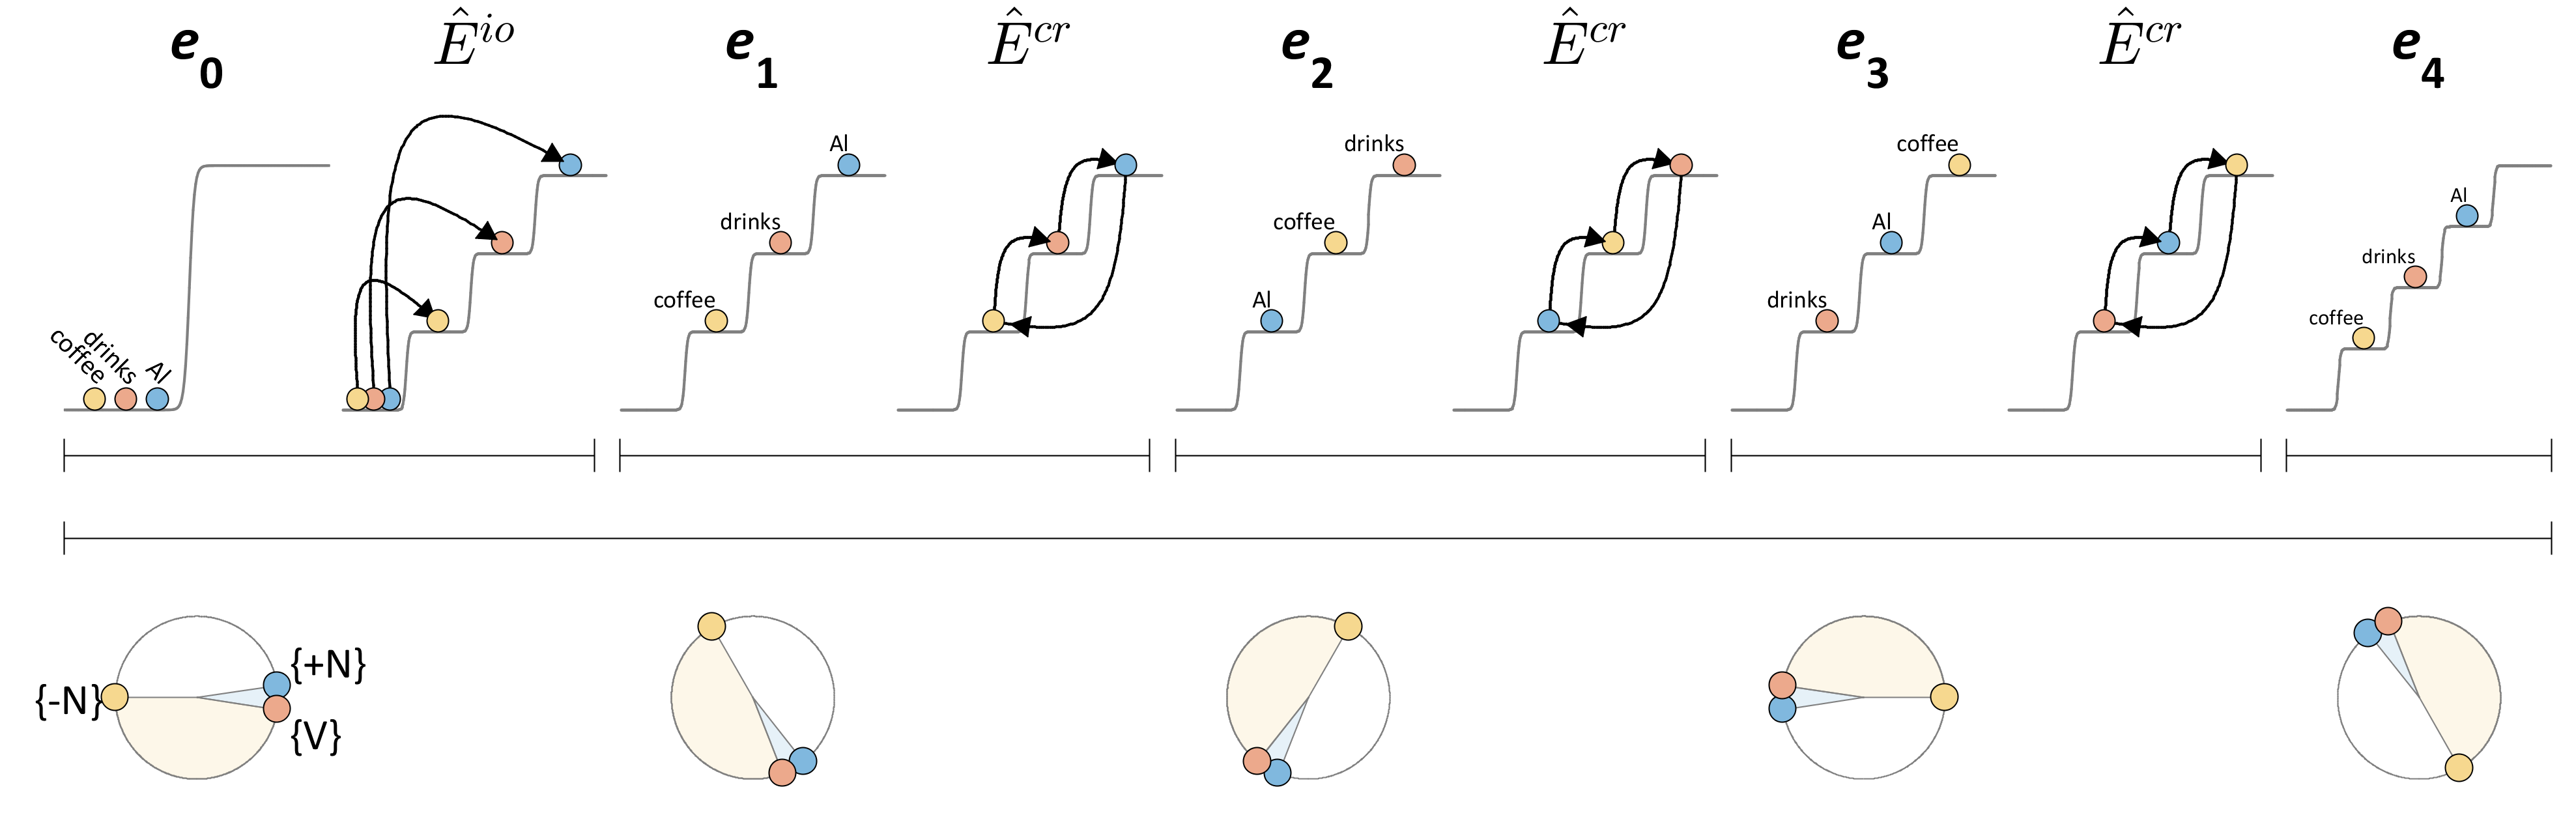
\includegraphics[width=\textwidth]{figures/Tilsen-img27.png}
\caption{\missingcaption}
\label{fig:}
\end{figure}
 

  In conventional approaches, there are diverse perspectives on how linearization (selection/ordering) and structure building (relational meaning) interact, but these are generally understood to create and operate on structures of connected objects. The o/el model provides an alternative framework for thinking about the interaction between relational meaning and temporal order, one specific to φ-organization, the other specific to e-organization. Because φ-epochs tend to span multiple e-epochs, it is not easy, nor even useful to combine them into a single space for visualization. One approach would be to map relative excitation to oscillator amplitude, in which case we can visualize the temporal evolution as below:

  
\begin{figure}
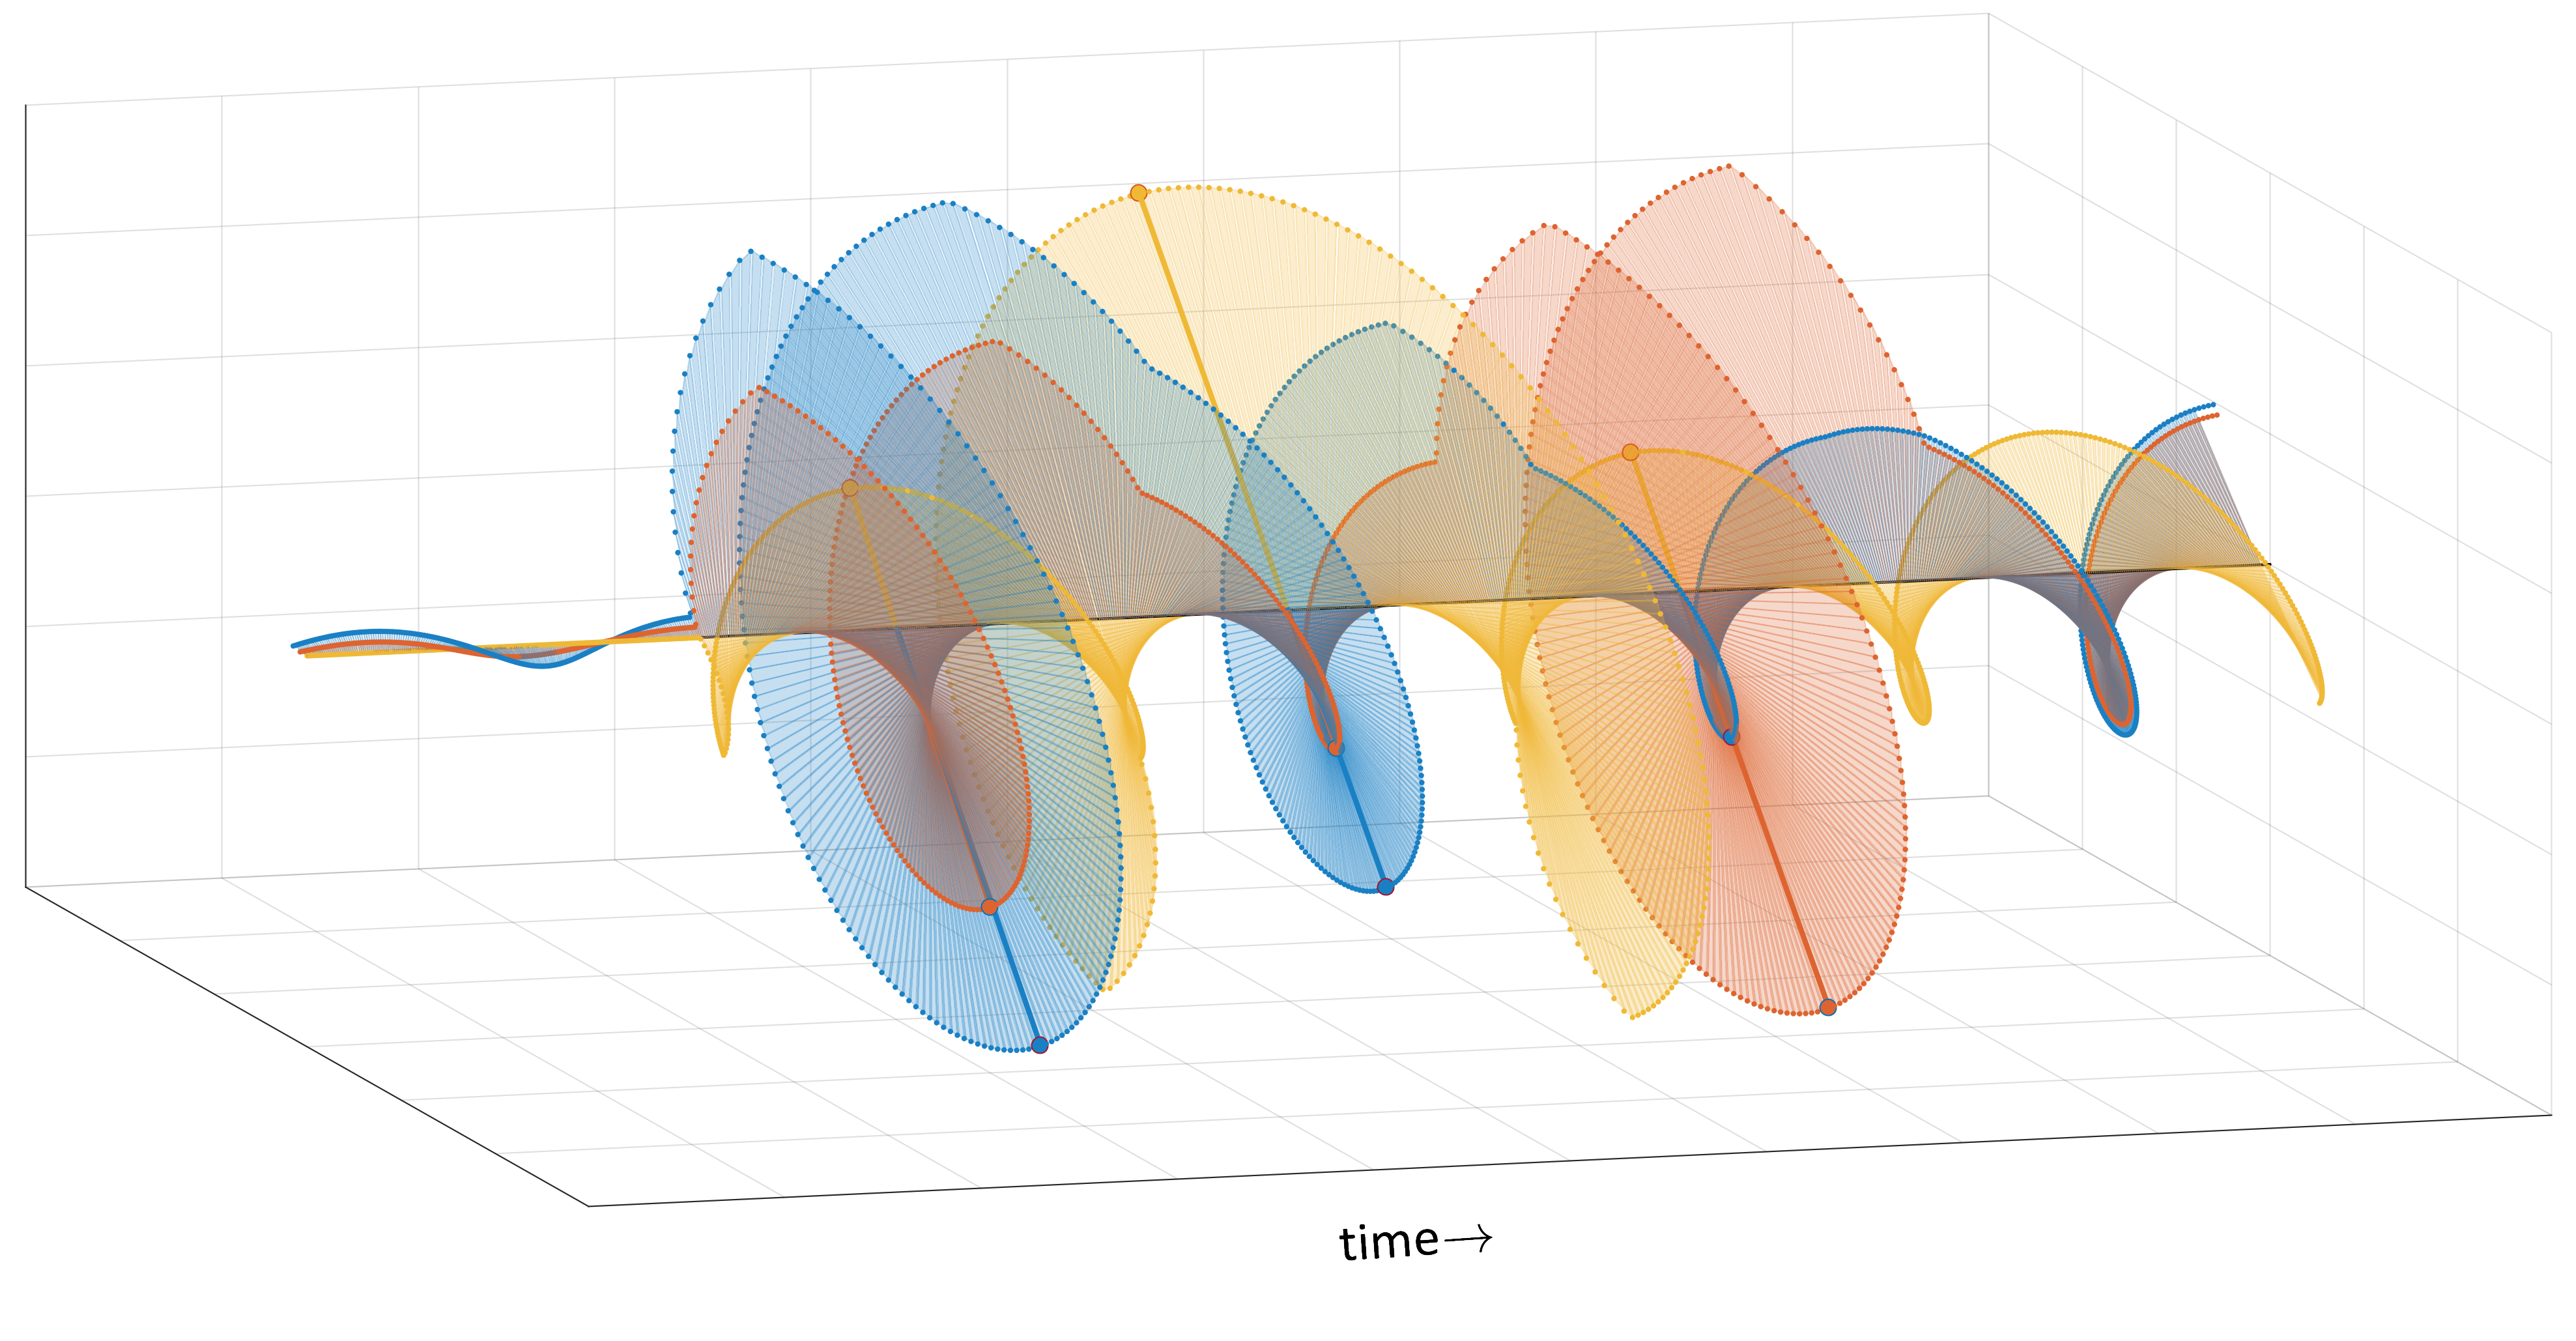
\includegraphics[width=\textwidth]{figures/Tilsen-img28.png}
\caption{\missingcaption}
\label{fig:}
\end{figure}
 

  This corkscrew visualization is too cluttered to be of much use, so instead we often juxtapose e-potential and φ{}-circle representations. These representations are analytical tools which encourage us to think differently about speech. Word order, instead of being a spatial arrangement of objects, is understood as a discontinuous trajectory in excitation space. Meaning relations, instead of being connections between objects, are experiences of stable relative phase differences between system oscillations.

\section{Conventions and terminology}

\textit{A}: order parameter of a system

\textit{S}: surroundings

θ, r: phase, radial amplitude of oscillatory component of order parameter
\textit{e}: excitation component of order parameter

φ: relative phase

c-system: concept system. written in square brackets, e.g. [coffee], [drink]

s-system: syntactic system. written in curly brackets, e.g. \{-N\}, \{V\}

cs-system or system: pair of resonating c- and s-systems, e.g. [drink]\{V\}, [coffee]\{-N\}

cs-systems in a stable configuration: {\textbar}drink coffee{\textbar}

Utterances: written italicized text, e.g. \textit{Al drinks coffee}

+φ-coupling/configuration: in-phase (attractive, proximal) relative phase-coupling/configuration

{}-φ-coupling/configuration: anti-phase (repulsive, distal) relative phase-coupling/configuration

+e-coupling: excitatory e-coupling

{}-e-coupling: inhibitory e-coupling

 $\widehat {{E}}$: e-organization operator
